\documentclass[12pt]{article}
   
\usepackage[utf8]{inputenc}
   \usepackage{graphicx}
   \usepackage{float}
   \usepackage{subcaption}
   %\usepackage{mathtools}
   \usepackage{amsmath}
   \usepackage{listings}
    \usepackage{xcolor}
    
    \definecolor{codegreen}{rgb}{0,0.6,0}
    \definecolor{codegray}{rgb}{0.5,0.5,0.5}
    \definecolor{codepurple}{rgb}{0.58,0,0.82}
    \definecolor{backcolour}{rgb}{0.95,0.95,0.92}
    
    \lstdefinestyle{codestyle}{
        backgroundcolor=\color{backcolour},   
        commentstyle=\color{codegreen},
        keywordstyle=\color{magenta},
        numberstyle=\tiny\color{codegray},
        stringstyle=\color{codepurple},
        basicstyle=\ttfamily\footnotesize,
        breakatwhitespace=false,         
        breaklines=true,                 
        captionpos=b,                    
        keepspaces=true,                 
        numbers=left,                    
        numbersep=5pt,                  
        showspaces=false,                
        showstringspaces=false,
        showtabs=false,                  
        tabsize=2
    }
    
    \lstset{style=codestyle}

   \addtolength{\hoffset}{-0.7in}
   \addtolength{\textheight}{1.5in}
   \addtolength{\textwidth}{1.5in}
   \addtolength{\voffset}{-1in}
%
% Title.
\title{EE230: Experiment 5\\
Observing frequency response of a filter in time domain}

% Author
\author{Hitesh Kandala, 180070023}

% begin the document.
\begin{document}

% make a title page.
\maketitle

\section{Overview of the experiment}

    \subsection{Aim of the experiment}
        The aim of the experiment is to observe frequency response of a High pass filter by implementing a sweep sine wave generator.
%%%%%%%%%%%%%%%%%%%%%%%%%%%%%%%%%%%%%%%%%%%%%%%%%%%%%%%%%%%%%%%%%%%%%%%%%%%%%%%%%%%%%%%%%%%%%%%%%
    \subsection{Theory}
        To measure frequency response, we need sweep sine wave generator (that
        generates sinusoidal signal whose frequency can be varied linearly keeping
        amplitude constant) as shown below.
        \begin{figure}[H]
            \centering
            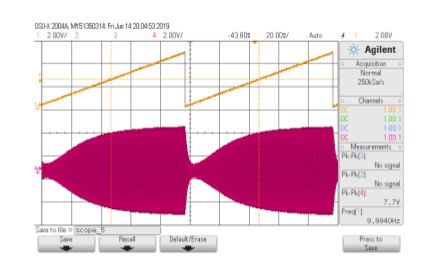
\includegraphics[width = 0.6\linewidth]{reports/lab5/HPF.png}
            \caption{HIGH PASS FILTER}
        \end{figure}
        \newpage
        \noindent
        Oscillators are circuits that produce periodic waveforms without any input signal.
        Fig. 2 demonstrates a basic negative feedback system in which $V_{IN}$ is the input voltage, $V_{OUT}$ is the output voltage from the amplifier block with gain A and $\beta$ as the feedback factor, that is fed back to the summing junction. E represents the error signal that is equal to the summation of the feedback factor and the input voltage.
        \begin{figure}[H]
            \centering
            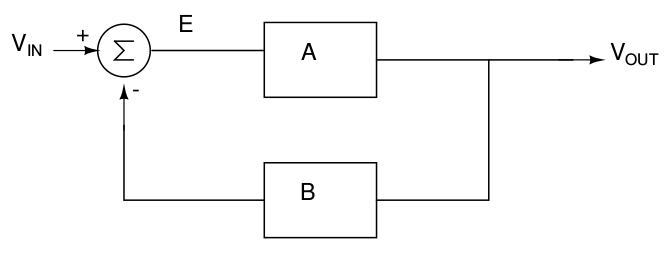
\includegraphics[width=0.5\linewidth]{reports/lab5/feedback.png}
            \caption{Block diagram of feedback network}
            \label{fig:loadcell}
        \end{figure}
        \begin{gather}
        	E = V_{IN} - \beta V_{OUT}\\
        	V_{OUT} = AE = A (V_{IN} - \beta V_{OUT})\\
        	A_f = \frac{V_{OUT}}{V_{IN}} = \frac{A}{1 + A\beta}
        \end{gather}
        \noindent
        When A$\beta = 1\angle - 180^o$ , the denominator term becomes 0 and the gain with feedback, becomes infinite. This means infinitesimal signal can provide an output voltage. When the condition for loop gain and phase shift is satisfied, the circuit produces output without an input signal. This is \textit{Barkhausen Criterion} for sustained oscillations.
        \\\\
        In practical circuits, however, it is found that for the loop gain A$\beta$, even if made equal to unity, the oscillations die out exponentially as the devices used for amplification are nonlinear in nature and cause the gain to reduce from their nominal value resulting in oscillations to cease. Hence; the loop gain A$\beta$ is made slightly greater than one to build up oscillations. The growing oscillations are then limited by the non-linearity of the circuit elements. The automatic gain control circuits are also often used to stabilise the amplitude of oscillations to result in less distortion.
        \subsubsection{Wien Bridge Oscillator}
            The Wien bridge oscillator is one of the simplest oscillators. Fig.2 shows the basic Wien bridge circuit configuration. OPAMP is used as the amplifying device and the Wien Bridge is used as the feedback element.
            \begin{figure}[H]
                \centering
                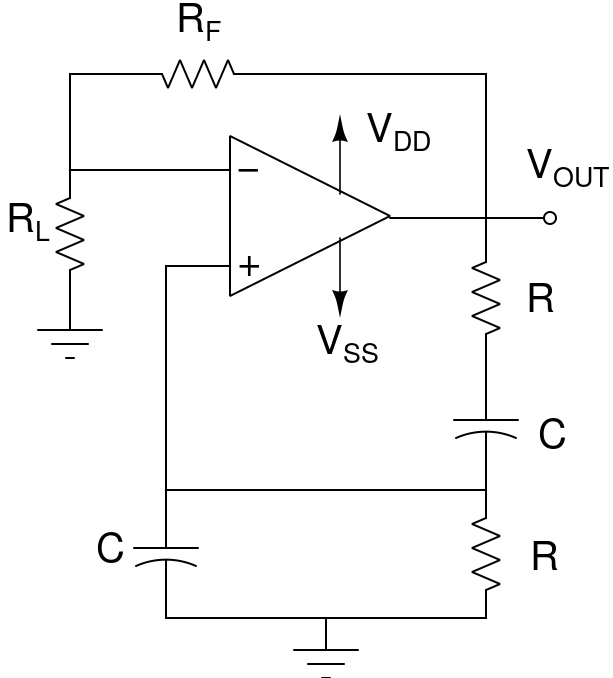
\includegraphics[width=0.4\linewidth]{reports/lab5/wien2.png}
                \caption{Wien Bridge Oscillator}
                \label{fig:instru}
            \end{figure}
            \noindent
            The OPAMP is used in non-inverting mode that provides a phase shift of $0^o$ . One can expect that the phase shift introduced by the feedback network also to be equal to $0^o$ at the frequency of oscillations. The frequency of oscillations is,
            \begin{equation}
                f = \frac{1}{2\pi RC}
            \end{equation}
            \noindent
            This condition comes from solving for $V_f$ i.e. the feedback voltage
            \begin{figure}[H]
                \centering
                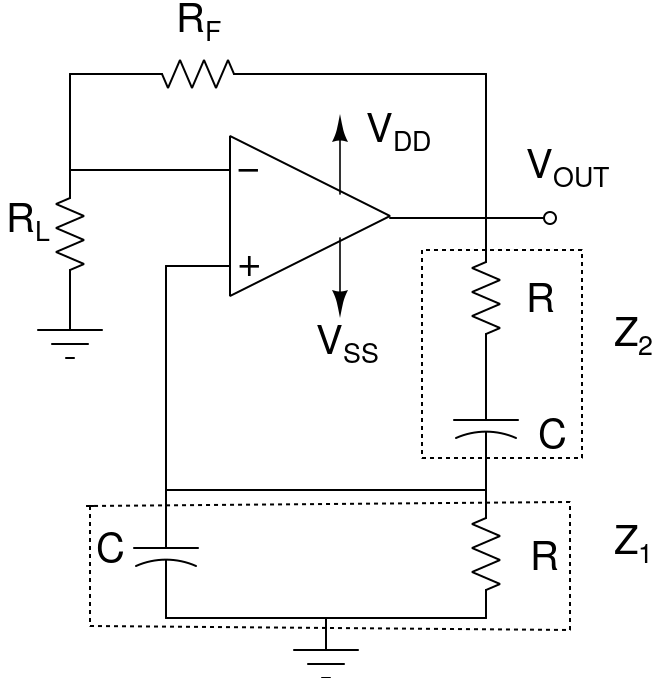
\includegraphics[width=0.4\linewidth]{reports/lab5/wien.png}
                \caption{Analysis of Wien Bridge Oscillator}
                \label{fig:instru}
            \end{figure}
            \noindent
            The feedback voltage is given by,
            \begin{equation}
                V_f = \frac{Z_1}{Z_1+Z_2}V_{OUT} 
            \end{equation}
            \noindent
            where,
            \begin{gather}
                Z_1 = \frac{R}{1+RCS}\\
                Z_2 = R + \frac{1}{CS}
            \end{gather}
            \noindent
            Substituting these values in Eq. 5 we get,
            \begin{equation}
                V_f = \frac{\frac{R}{1+RCS}}{\frac{R}{1+RCS}+R + \frac{1}{CS}}V_{OUT} 
            \end{equation}
            \noindent
            Substituting the value of S = $j\omega$ and simplifying we get,
            \begin{equation}
                V_f = \frac{j\omega RC}{1+3j\omega RC - \omega^2R^2C^2}V_{OUT}
            \end{equation}
            \noindent
            To ensure phase shift of $0^o$ by the feedback network, $1 - \omega^2R^2C^2 = 0$, which leads to
            \begin{equation}
                \omega = \frac{1}{RC} \rightarrow f = \frac{1}{2\pi RC}
            \end{equation}
            \noindent
            This happens for
            \begin{equation}
                V_f = \frac{V_{OUT}}{3} 
            \end{equation}
            \noindent
            This implies that the non-inverting gain of the amplifier should be slightly greater than 3 so that the loop gain condition is satisfied.
 %%%%%%%%%%%%%%%%%%%%%%%%%%%%%%%%%%%%%%%%%%%%%%%%%%%%%%%%%%%%%%%%%%%%%%%%%%%%%%%%%%%%%%%%%%%%%%%%           
\section{Experimental results}
    
    \textbf{Procedure}
        \begin{itemize}
            \item The oscillating part of the Wein Bridge Oscillator was assembled and Bode plots of amplitude and frequency response were plotted with frequency ranging from 100Hz to 30kHz for $10V_{p-p}$ sine wave input.
            \item The Wien Bridge Oscillator was constructed. potentiometer at $R_5$ was adjusted to get sustained sinusoidal oscillations at the output. 
            \item  We then aimed to vary  $R_1$ and $R_2$ with voltage. For this we set up a different circuit with an LDR and op-amp, and measure $R_{out}$ of LDR with changes in input voltage.
            \item To generate sweep we connected $LED-LDR's$ in place of $R_1$ and $R_2$ of Wien Bridge Oscillator.Hence, now the frequency was dependent on resistance controlled by input frequency.
            \item  A negative feedback loop was added so the the amplitude remains same with variation in frequency caused due to non-idealities of OP-AMP. 
            \item We now connect this Sweep Generator to the second order Sallen Key high pass filter circuit and observe voltage wave-forms on the DSO.
        \end{itemize}
%%%%%%%%%%%%%%%%%%%%%%%%%%%%%%%%%%%%%%%%%%%%%%%%%%%%%%%%%%%%%%%%%%%%%%%%%%%%%%%%%%%%%%%%%%%%%%%%%%%%%%
    \subsection{Non-inverting Feedback Network of Wien Bridge Oscillator}
            
        \noindent
        \textbf{Observations and Inferences}\\
        
        \noindent
        The feedback network is shown below:
        \begin{figure}[H]
            \centering
            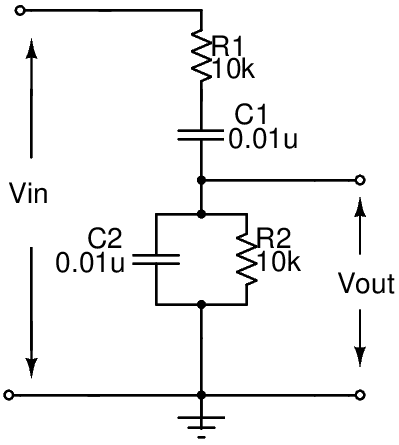
\includegraphics[width = 0.4\linewidth]{reports/lab5/p1.png}
            \caption{Positive feedback network of Wien Bridge Oscillator}
        \end{figure}
        \noindent
        The $V_{out}$ vs $V_{in}$ relation is given by equation 3,
        \\\\
        \noindent
        The waveform of $V_{out}$ for different frequencies on application of a 10 $V_{p-p}$ sine wave input is shown below:
        \begin{figure}[H]
            \centering
            \begin{subfigure}{.5\textwidth}
                \centering
                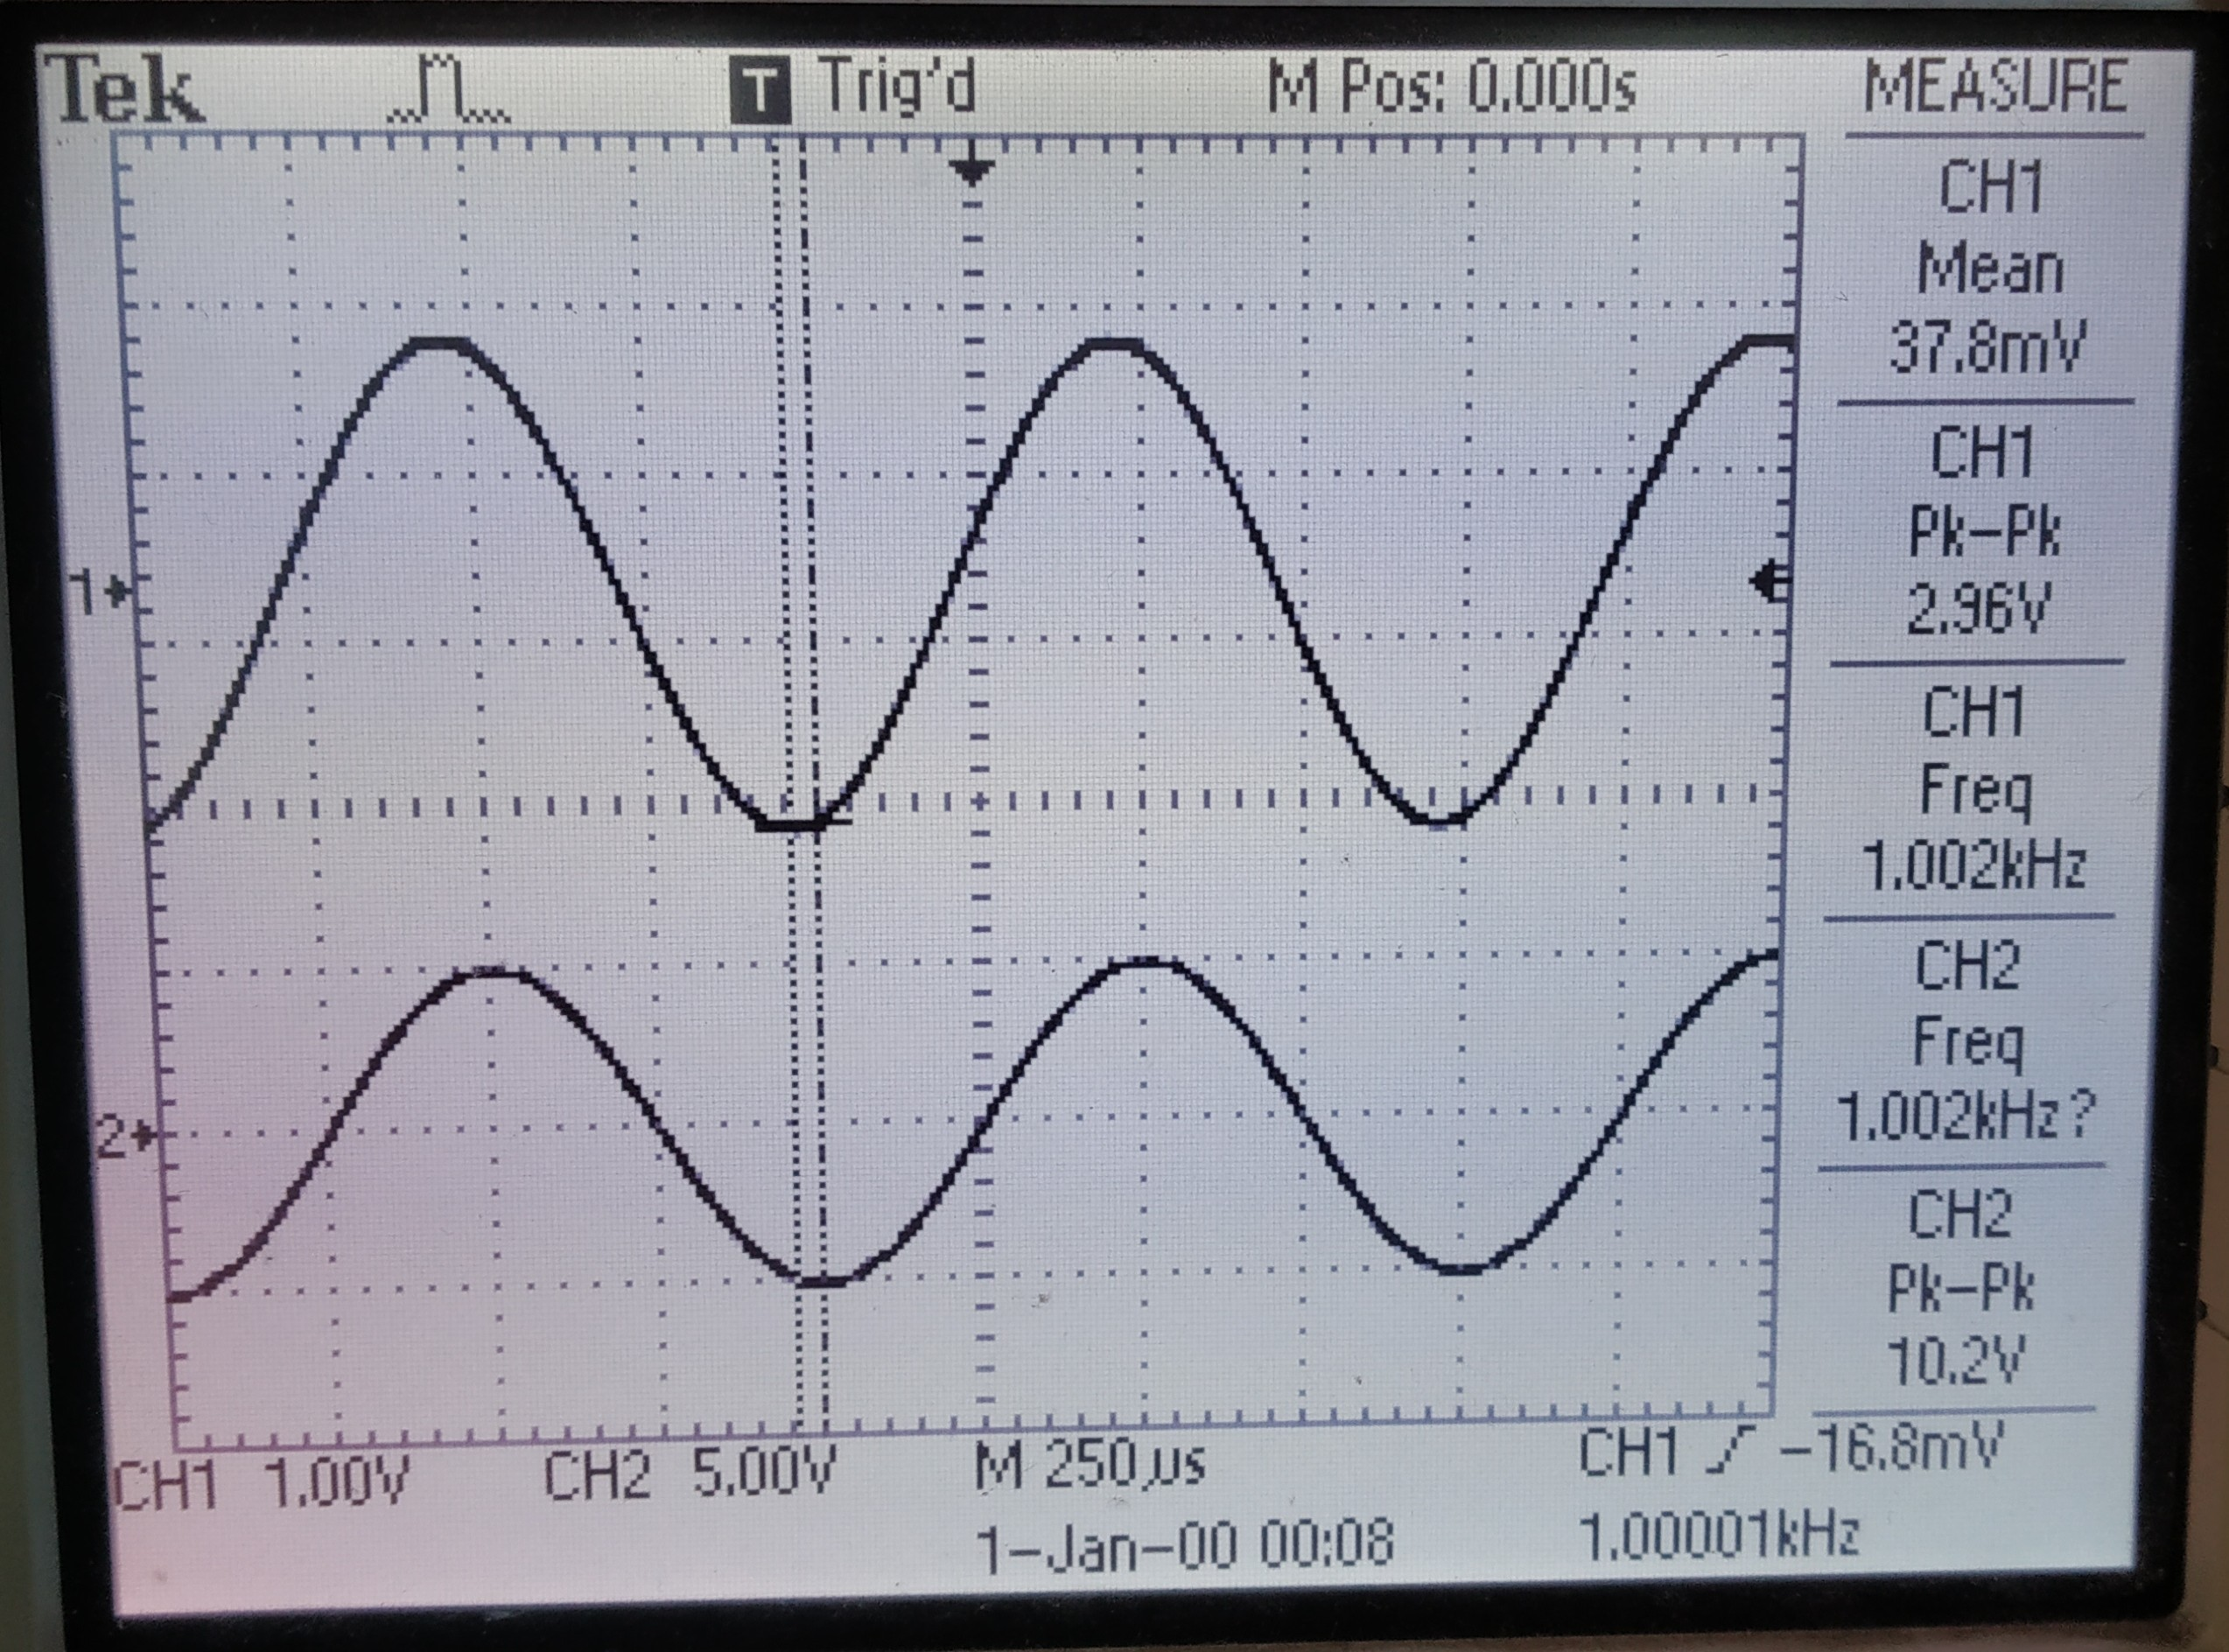
\includegraphics[width=70mm]{reports/lab5/firstpart_1khz.jpg}
                \caption{f = 1kHz}
            \end{subfigure}%
            \begin{subfigure}{.5\textwidth}
                \centering
                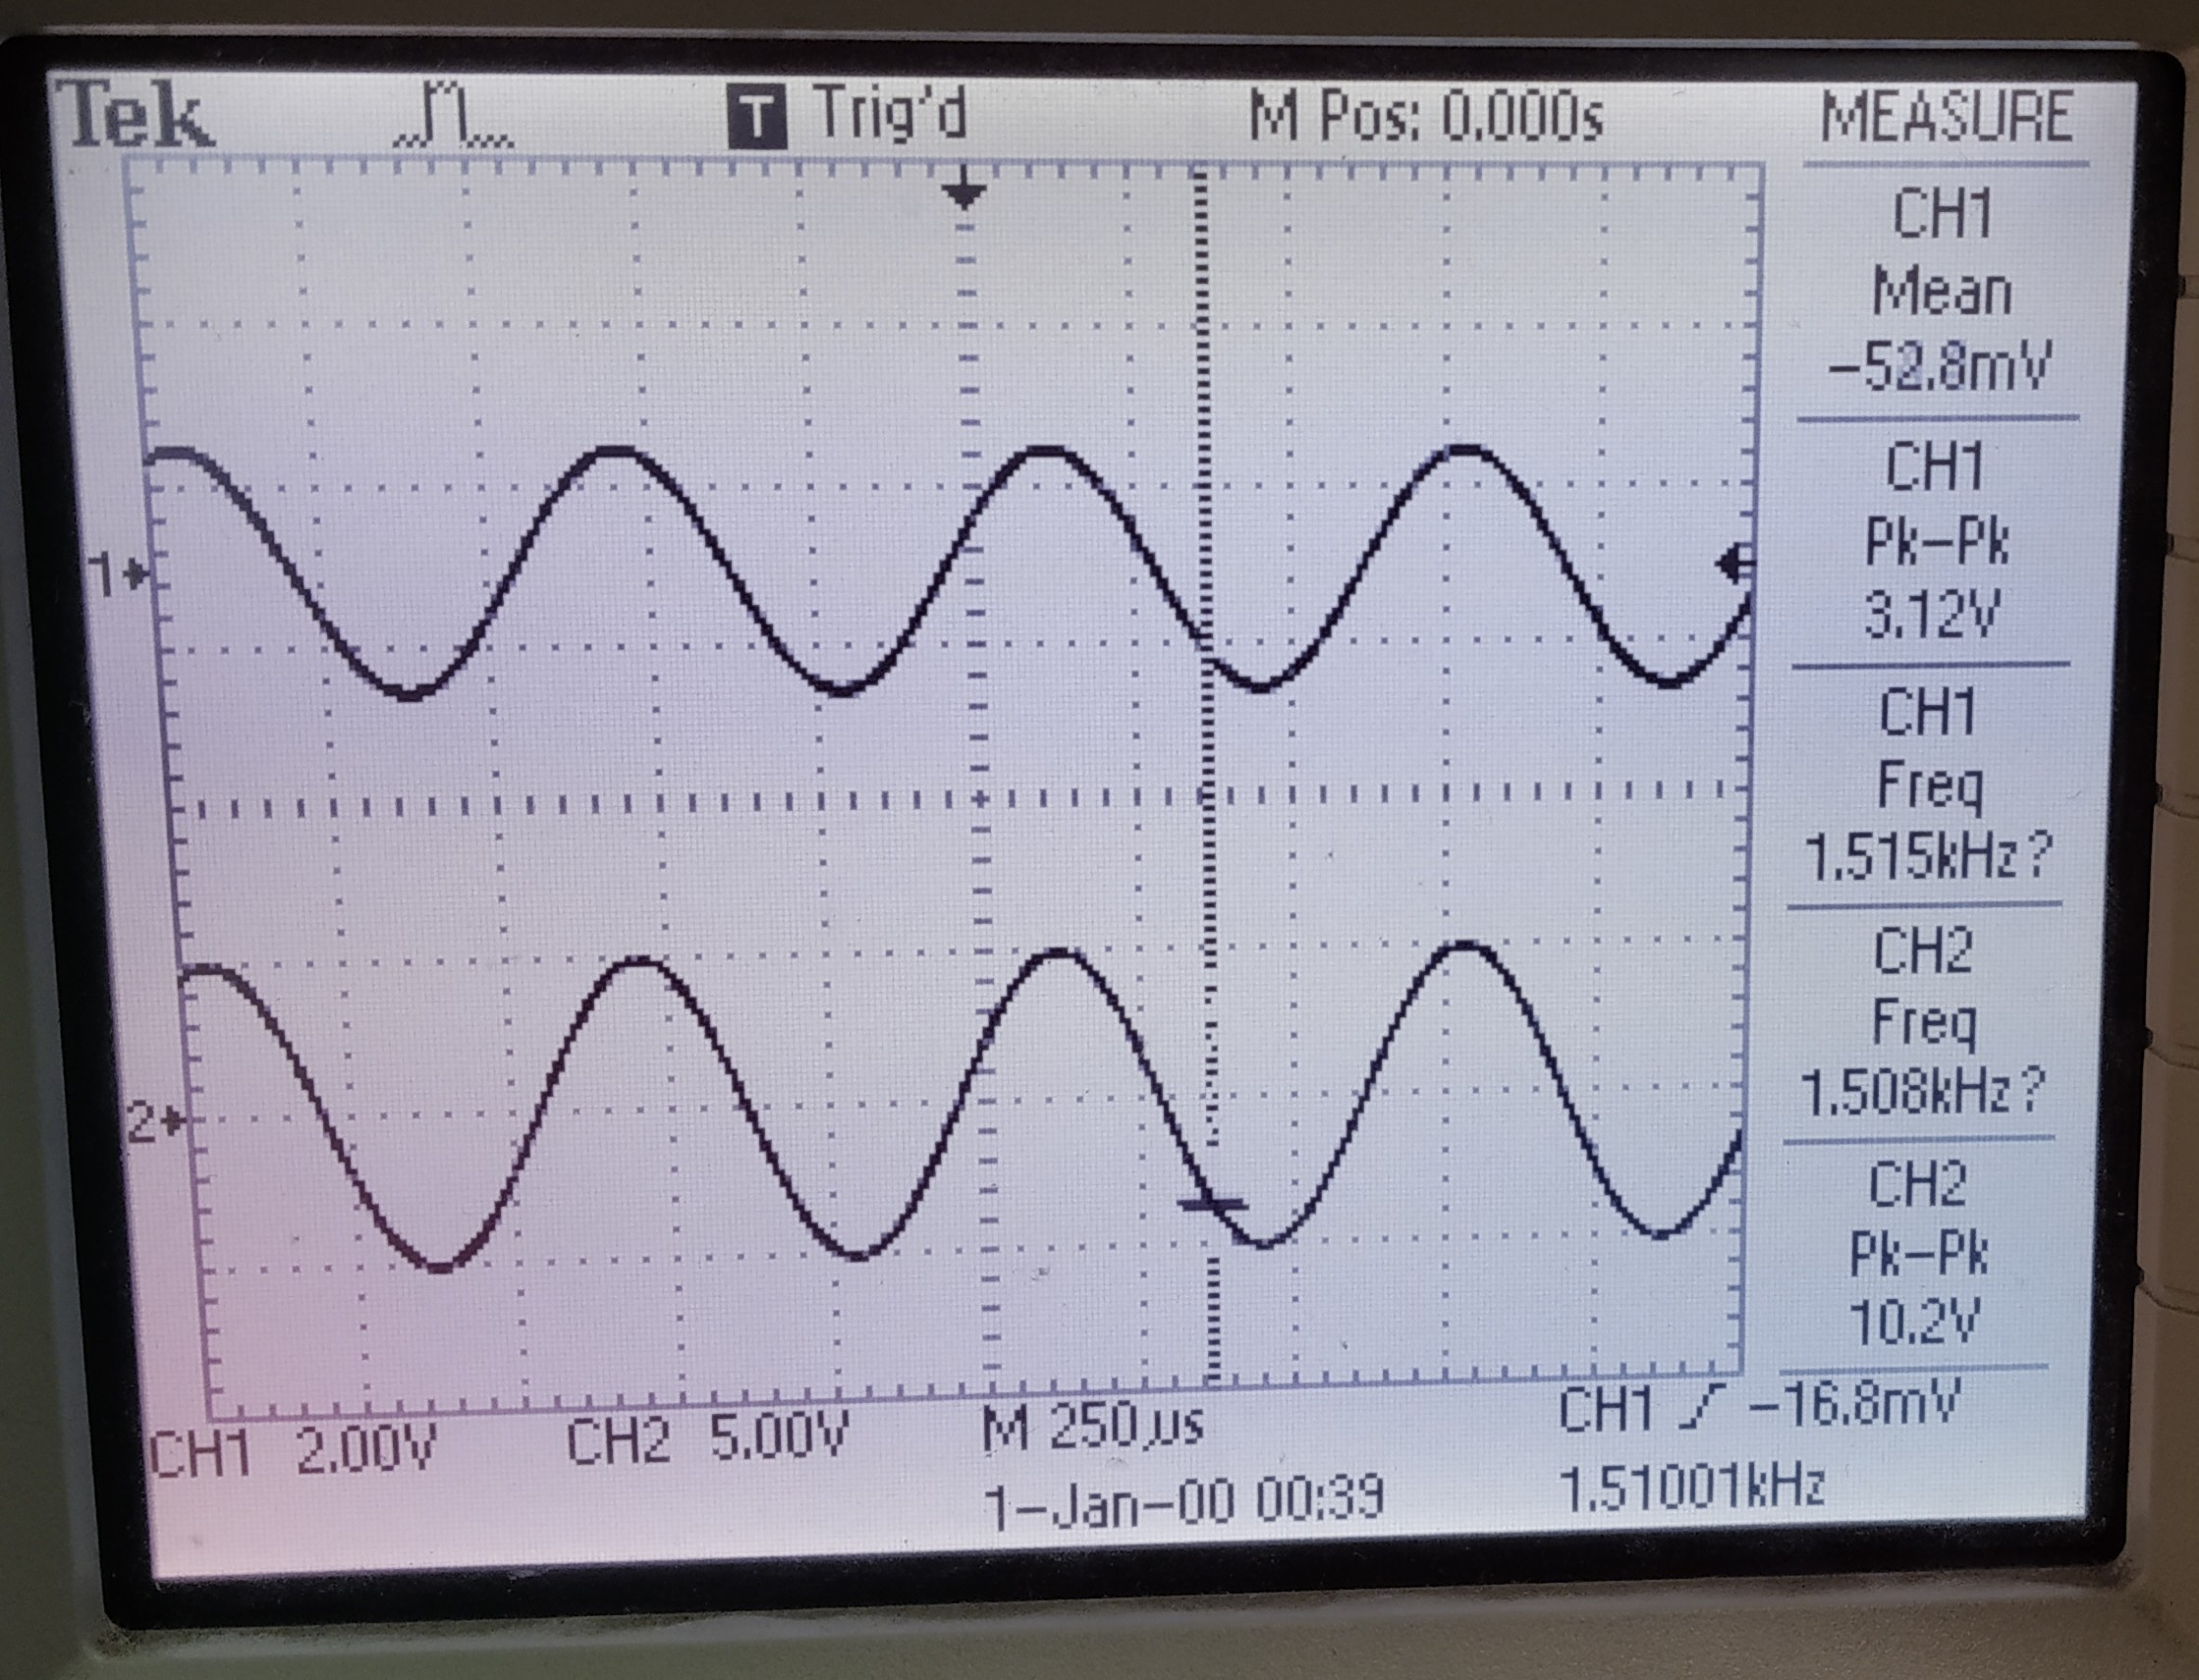
\includegraphics[width=70mm]{reports/lab5/firstpart_1_51khz.jpg}
                \caption{f = 1.51kHz}
            \end{subfigure}%
        \end{figure}
        \begin{figure}[H]
            \centering
            \begin{subfigure}{.5\textwidth}
                \centering
                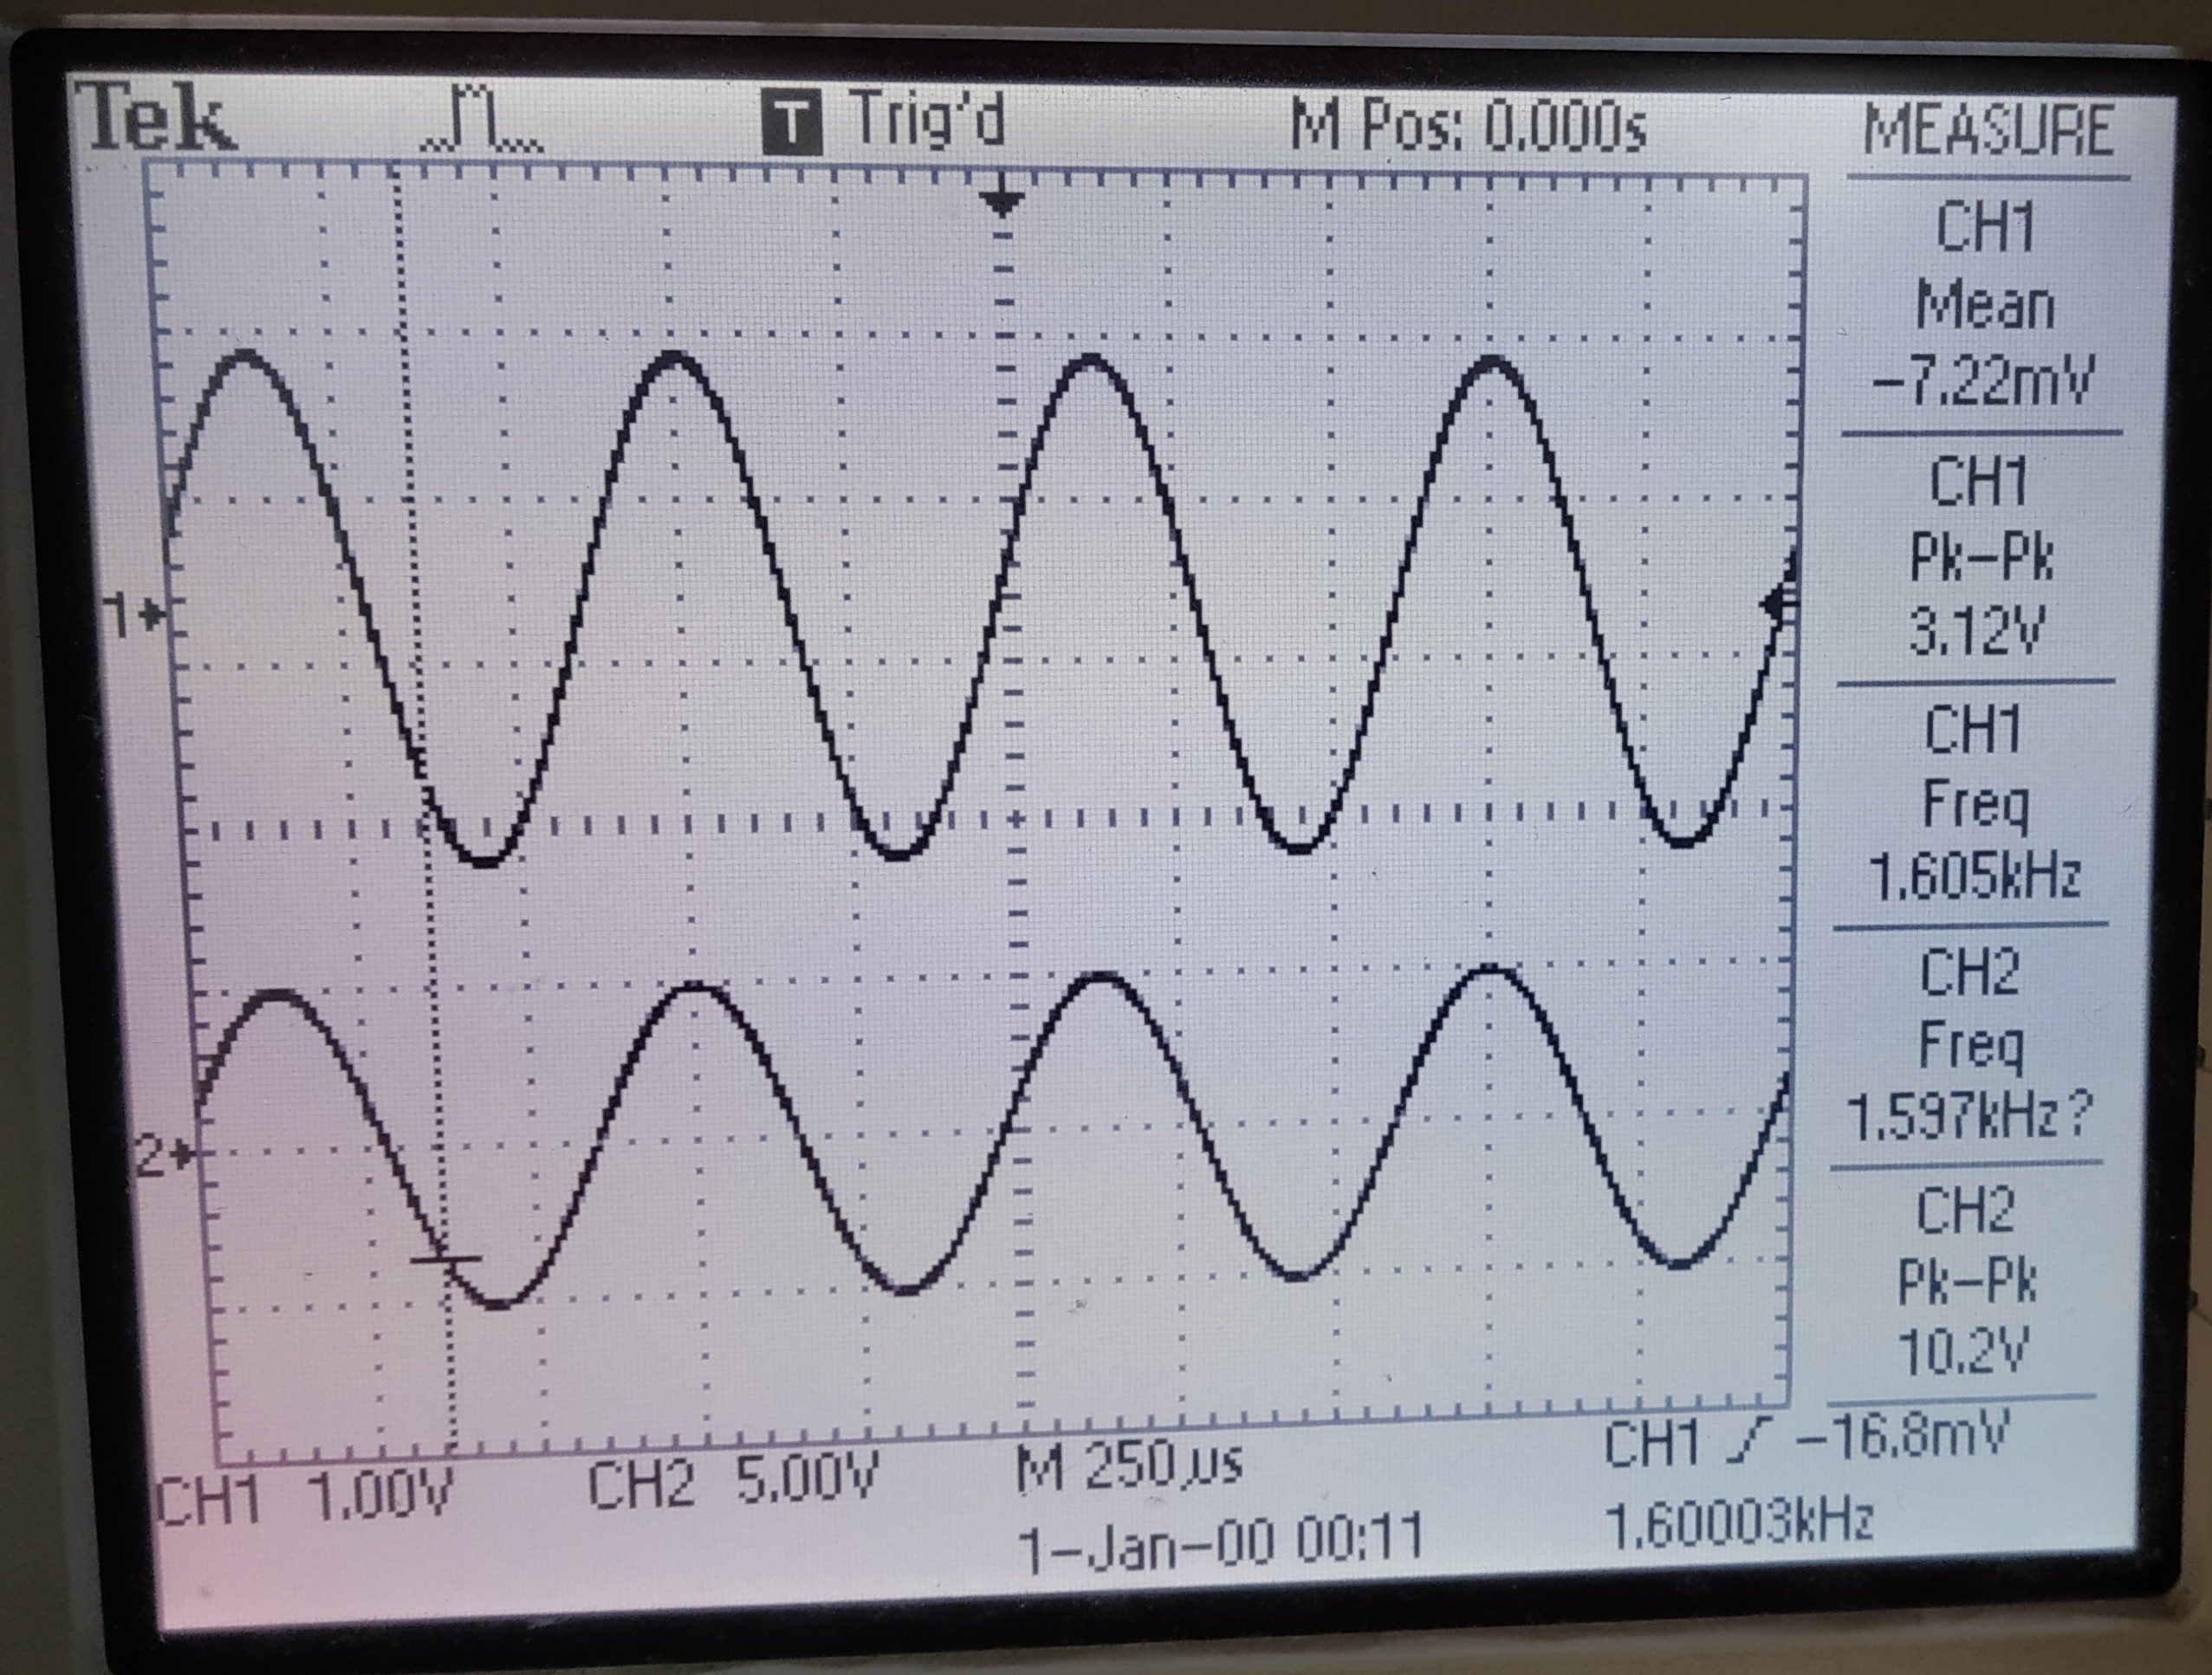
\includegraphics[width=70mm]{reports/lab5/firstpart_1_6khz.jpg}
                \caption{f = 1.6kHz}
            \end{subfigure}%
            \begin{subfigure}{.5\textwidth}
                \centering
                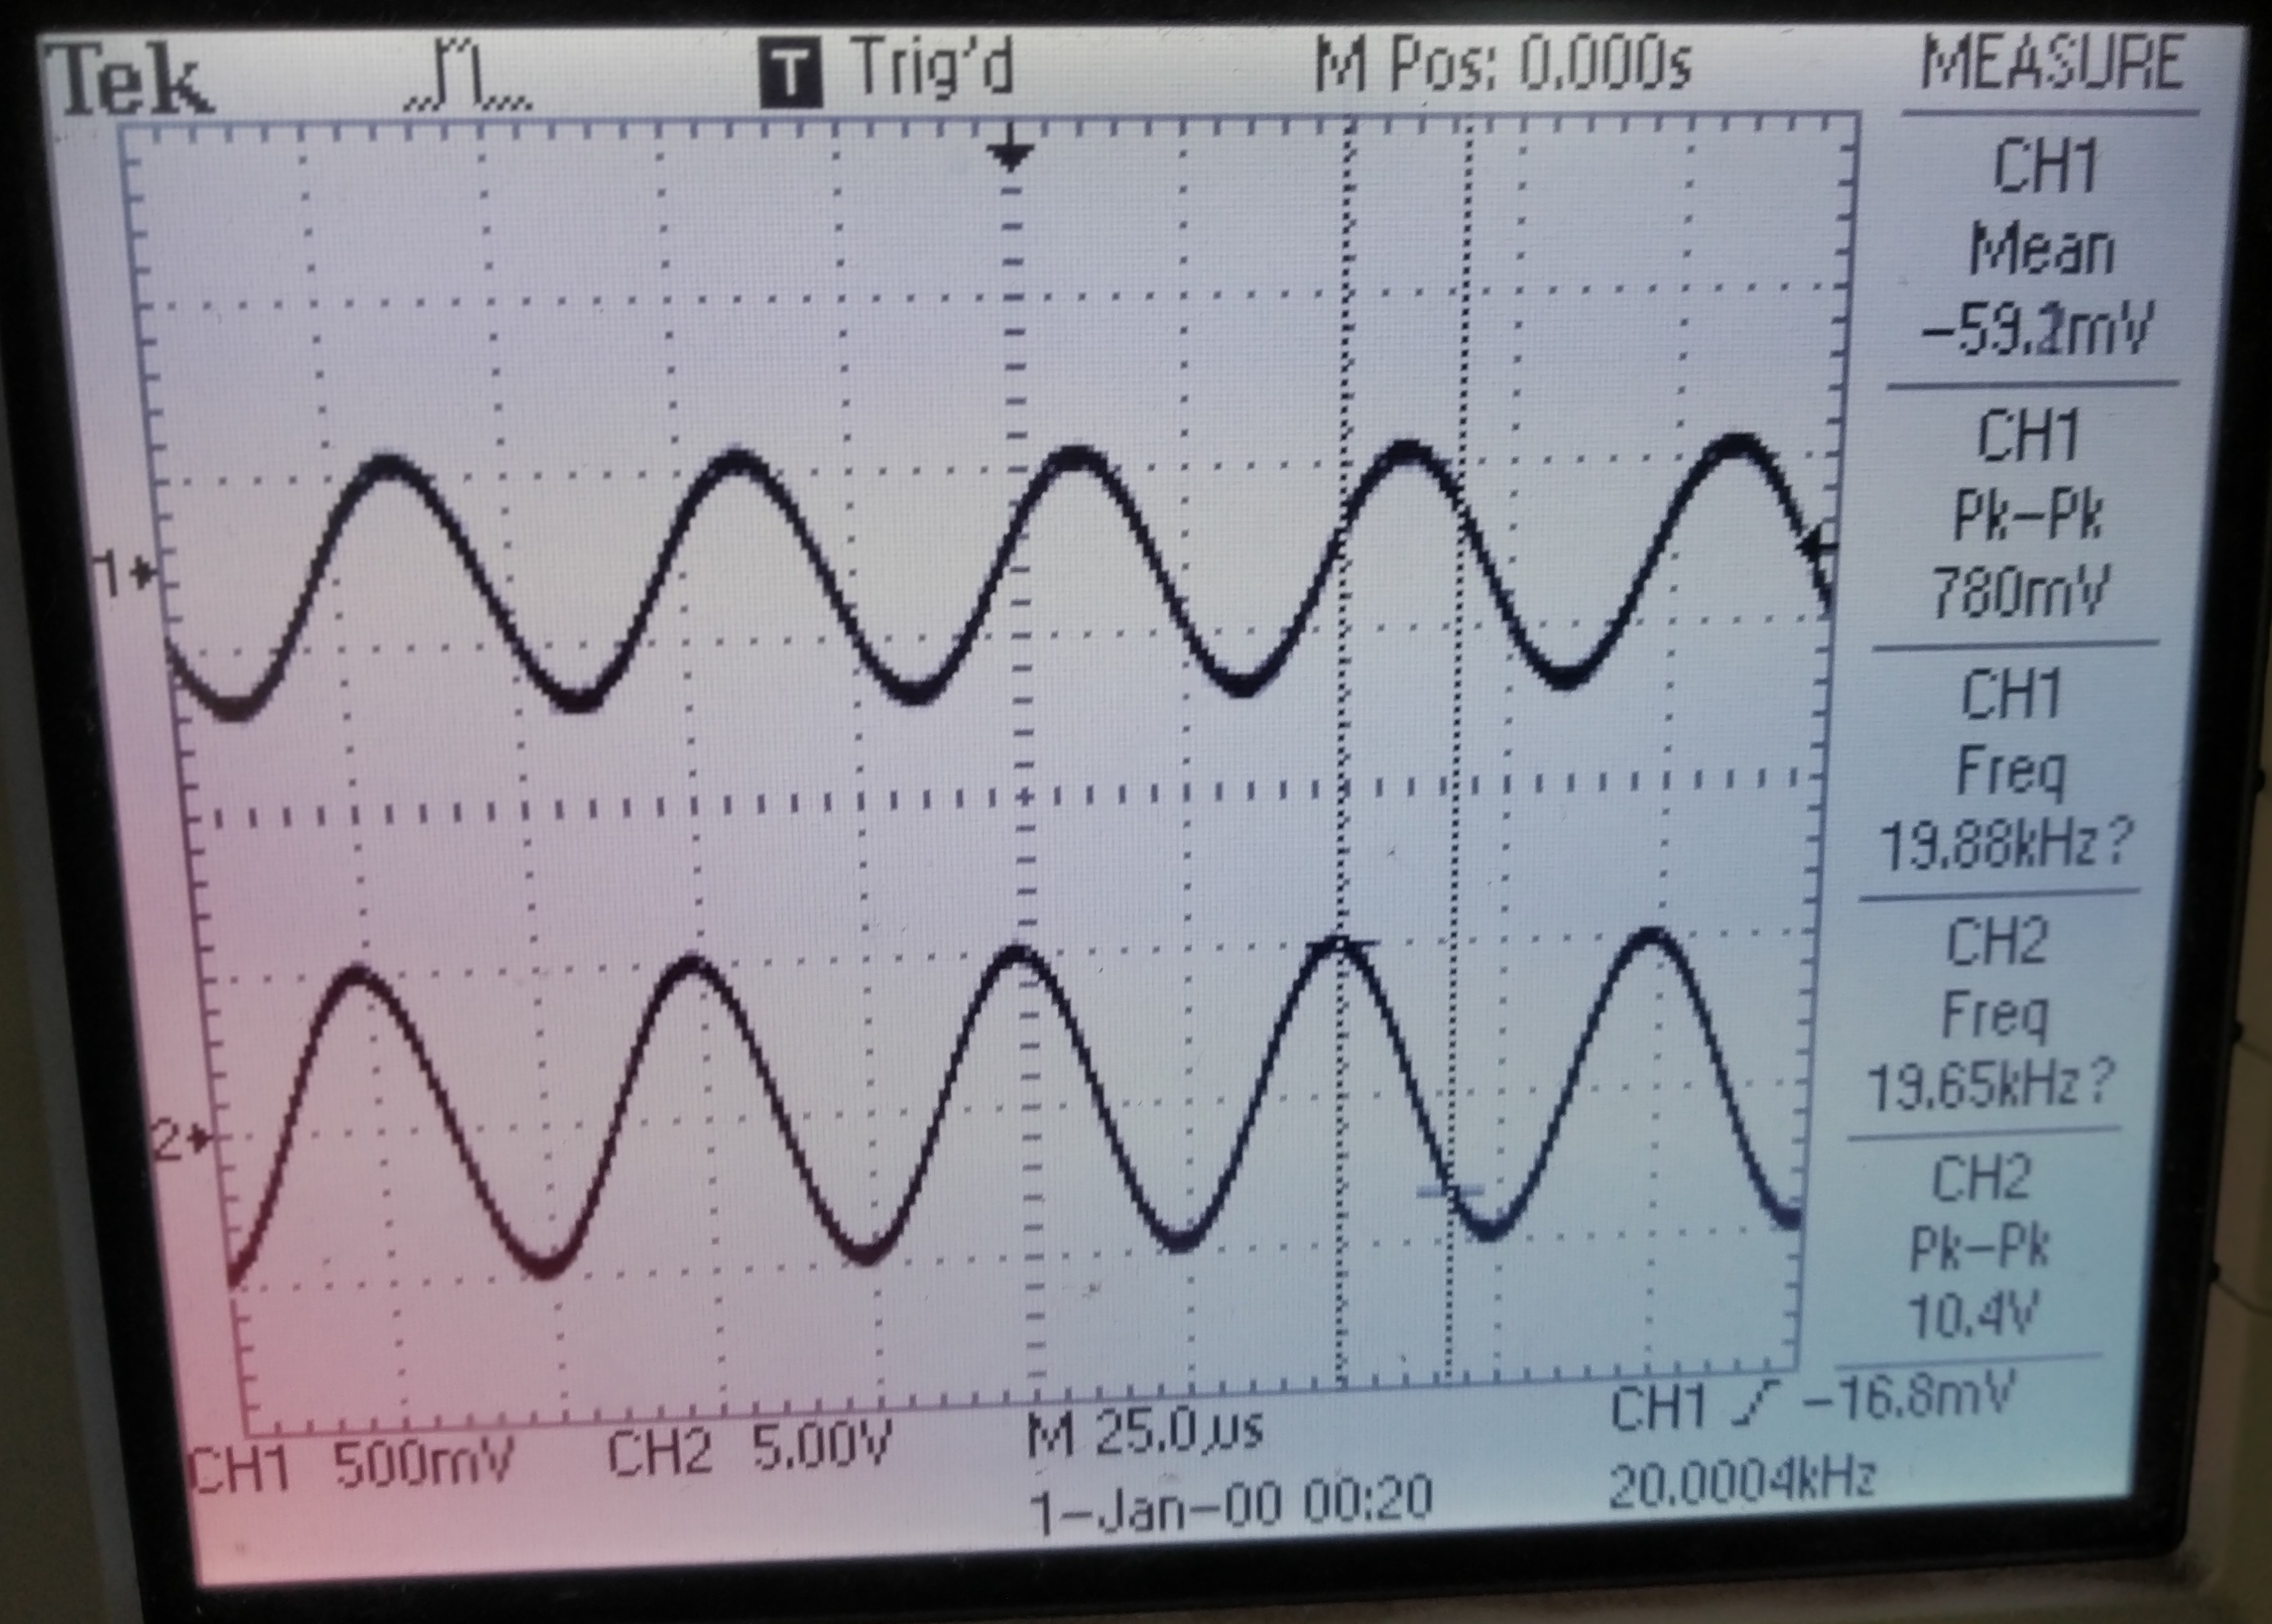
\includegraphics[width=70mm]{reports/lab5/firstpart_20khz.jpg}
                \caption{f = 20kHz}
            \end{subfigure}%
        \end{figure}
        \noindent
        The magnitude Bode plot obtained for the above circuit is as plotted below:\\\\
        % "Insert the axes information here"
        \begin{minipage}{\linewidth}
            \centering
            \begin{minipage}{0.4\linewidth}
                \begin{table}[H]
                    \centering
                    \begin{tabular}{|c|l|l|}
                    \hline
                        $\omega$(kHz) &$V_{out}$ (V)&$V_{in} (V)$\\ \hline
                        0.1	&	0.632	&	10.2	\\	\hline
                        0.5	&	2.32	&	10.2	\\	\hline
                        0.9	&	2.88	&	10.2	\\	\hline
                        1	&	2.96	&	10.2	\\	\hline
                        1.2	&	3.04	&	10.2	\\	\hline
                        1.4	&	3.12	&	10.2	\\	\hline
                        1.53	&	3.12	&	10.2	\\	\hline
                        1.59	&	3.12	&	10.2	\\	\hline
                        1.8	&	3.12	&	10.2	\\	\hline
                        2.2	&	3.04	&	10.2	\\	\hline
                        3	&	2.88	&	10.6	\\	\hline
                        10	&	1.44	&	10.6	\\	\hline
                        15	&	1.02	&	10.4	\\	\hline
                        20	&	0.78	&	10.4	\\	\hline
                        30	&	0.512	&	10.4	\\	\hline
                    \end{tabular}
                    \caption{Observation Table}
                    \label{tab:my_label}
                \end{table}
            \end{minipage}
            \hspace{0.02\linewidth}
            \begin{minipage}{0.56\linewidth}
                \begin{figure}[H]
                    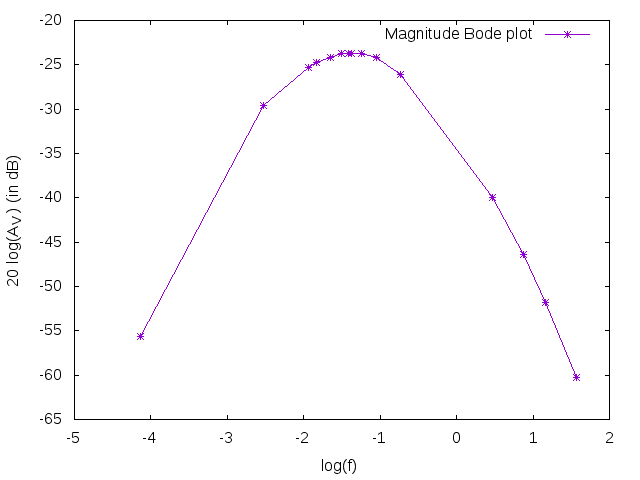
\includegraphics[width=\linewidth]{reports/lab5/mag.png}
                    \caption{amplitude response}
                    \label{Va_0_yt}
                \end{figure}
            \end{minipage}
        \end{minipage}
        \\\\
        \\\\
        \noindent
        The corresponding phase Bode plot is shown below.\\
        \begin{minipage}{\linewidth}
            \centering
            \begin{minipage}{0.4\linewidth}
                \begin{table}[H]
                    \centering
                    \begin{tabular}{|c|l|l|}
                    \hline
                        $\omega$(kHz) &$\Delta t$ (V)&$\phi \deg$\\ \hline
                        0.1	&	1800	&	64.8	\\	\hline
                        0.5	&	220	&	39.6	\\	\hline
                        1	&	40	&	14.4	\\	\hline
                        1.59	&	0	&	0	\\	\hline
                        1.8	&	-10	&	-6.48	\\	\hline
                        3	&	-26	&	-28.08	\\	\hline
                        10	&	-18	&	-64.8	\\	\hline
                        15	&	-12	&	-64.8	\\	\hline
                        20	&	-10	&	-72	\\	\hline
                        30	&	-7	&	-75.6	\\	\hline
                    \end{tabular}
                    \caption{Observation Table}
                    \label{tab:my_label}
                \end{table}
            \end{minipage}
            \hspace{0.02\linewidth}
            \begin{minipage}{0.56\linewidth}
                \begin{figure}[H]
                    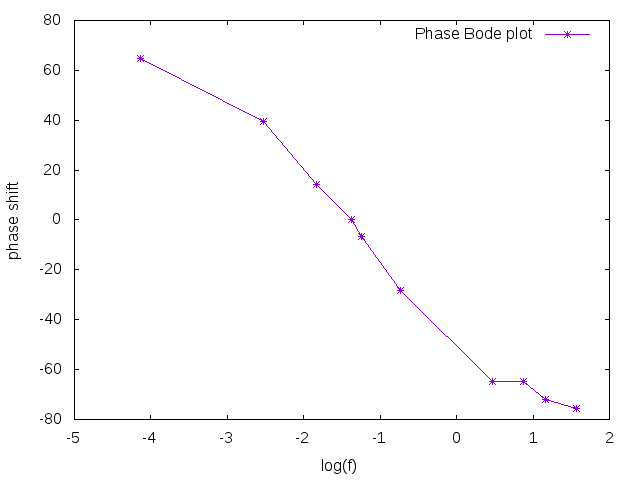
\includegraphics[width=\linewidth]{reports/lab5/phase.png}
                    \caption{phase response}
                    \label{Va_0_yt}
                \end{figure}
            \end{minipage}
        \end{minipage}
        \\\\
        \noindent
        $\ast$ The maximum gain obtained from magnitude bode plot is 0.305 at the frequency of 1.59kHz.
        \\\\
        \noindent
        $\ast$ The phase difference between $V_{in}$ and $V_{out}$ for maximum gain is 0.
%%%%%%%%%%%%%%%%%%%%%%%%%%%%%%%%%%%%%%%%%%%%%%%%%%%%%%%%%%%%%%%%%%%%%%%%%%%%%%%%%%%%%%%%%%%%%%%%%%%%%%%%   
    \subsection{Wien Bridge Oscillator}
    
        \noindent
        \textbf{Observations and Inferences}\\
        
        \noindent
        % The circuit of Wien Bridge Oscillator with its positive feedback network is shown below:
        \begin{figure}[H]
            \centering
            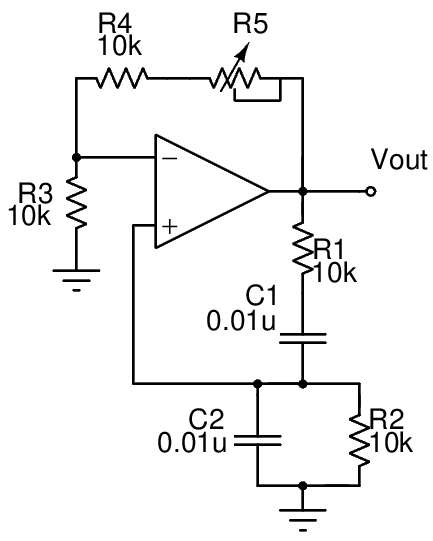
\includegraphics[width = 0.4\linewidth]{reports/lab5/p2.png}
            \caption{Circuit of wien bridge oscillator}
        \end{figure}
        \noindent
        The op-amp used in the above circuit is TL084 and the ideal values of the passive elements used are $R_1 = R_2 = 10k\Omega$, $C_1 = C_2 = 0.01\mu F$, $R_3 = R_4 = 10k\Omega$, $R_5 = 100k\Omega$ pot with +12V and -12V supply.\\\\
        \noindent
        Therefore the theoretical value of frequency of the Wien Bridge Osclillator is
        \begin{align}
            f &= \frac{1}{2\pi RC}\\
              &= \frac{1}{2\pi \times10k\times0.01\mu F}\\
              &= 1.591kHz
        \end{align}
        \begin{figure}[H]
            \centering
            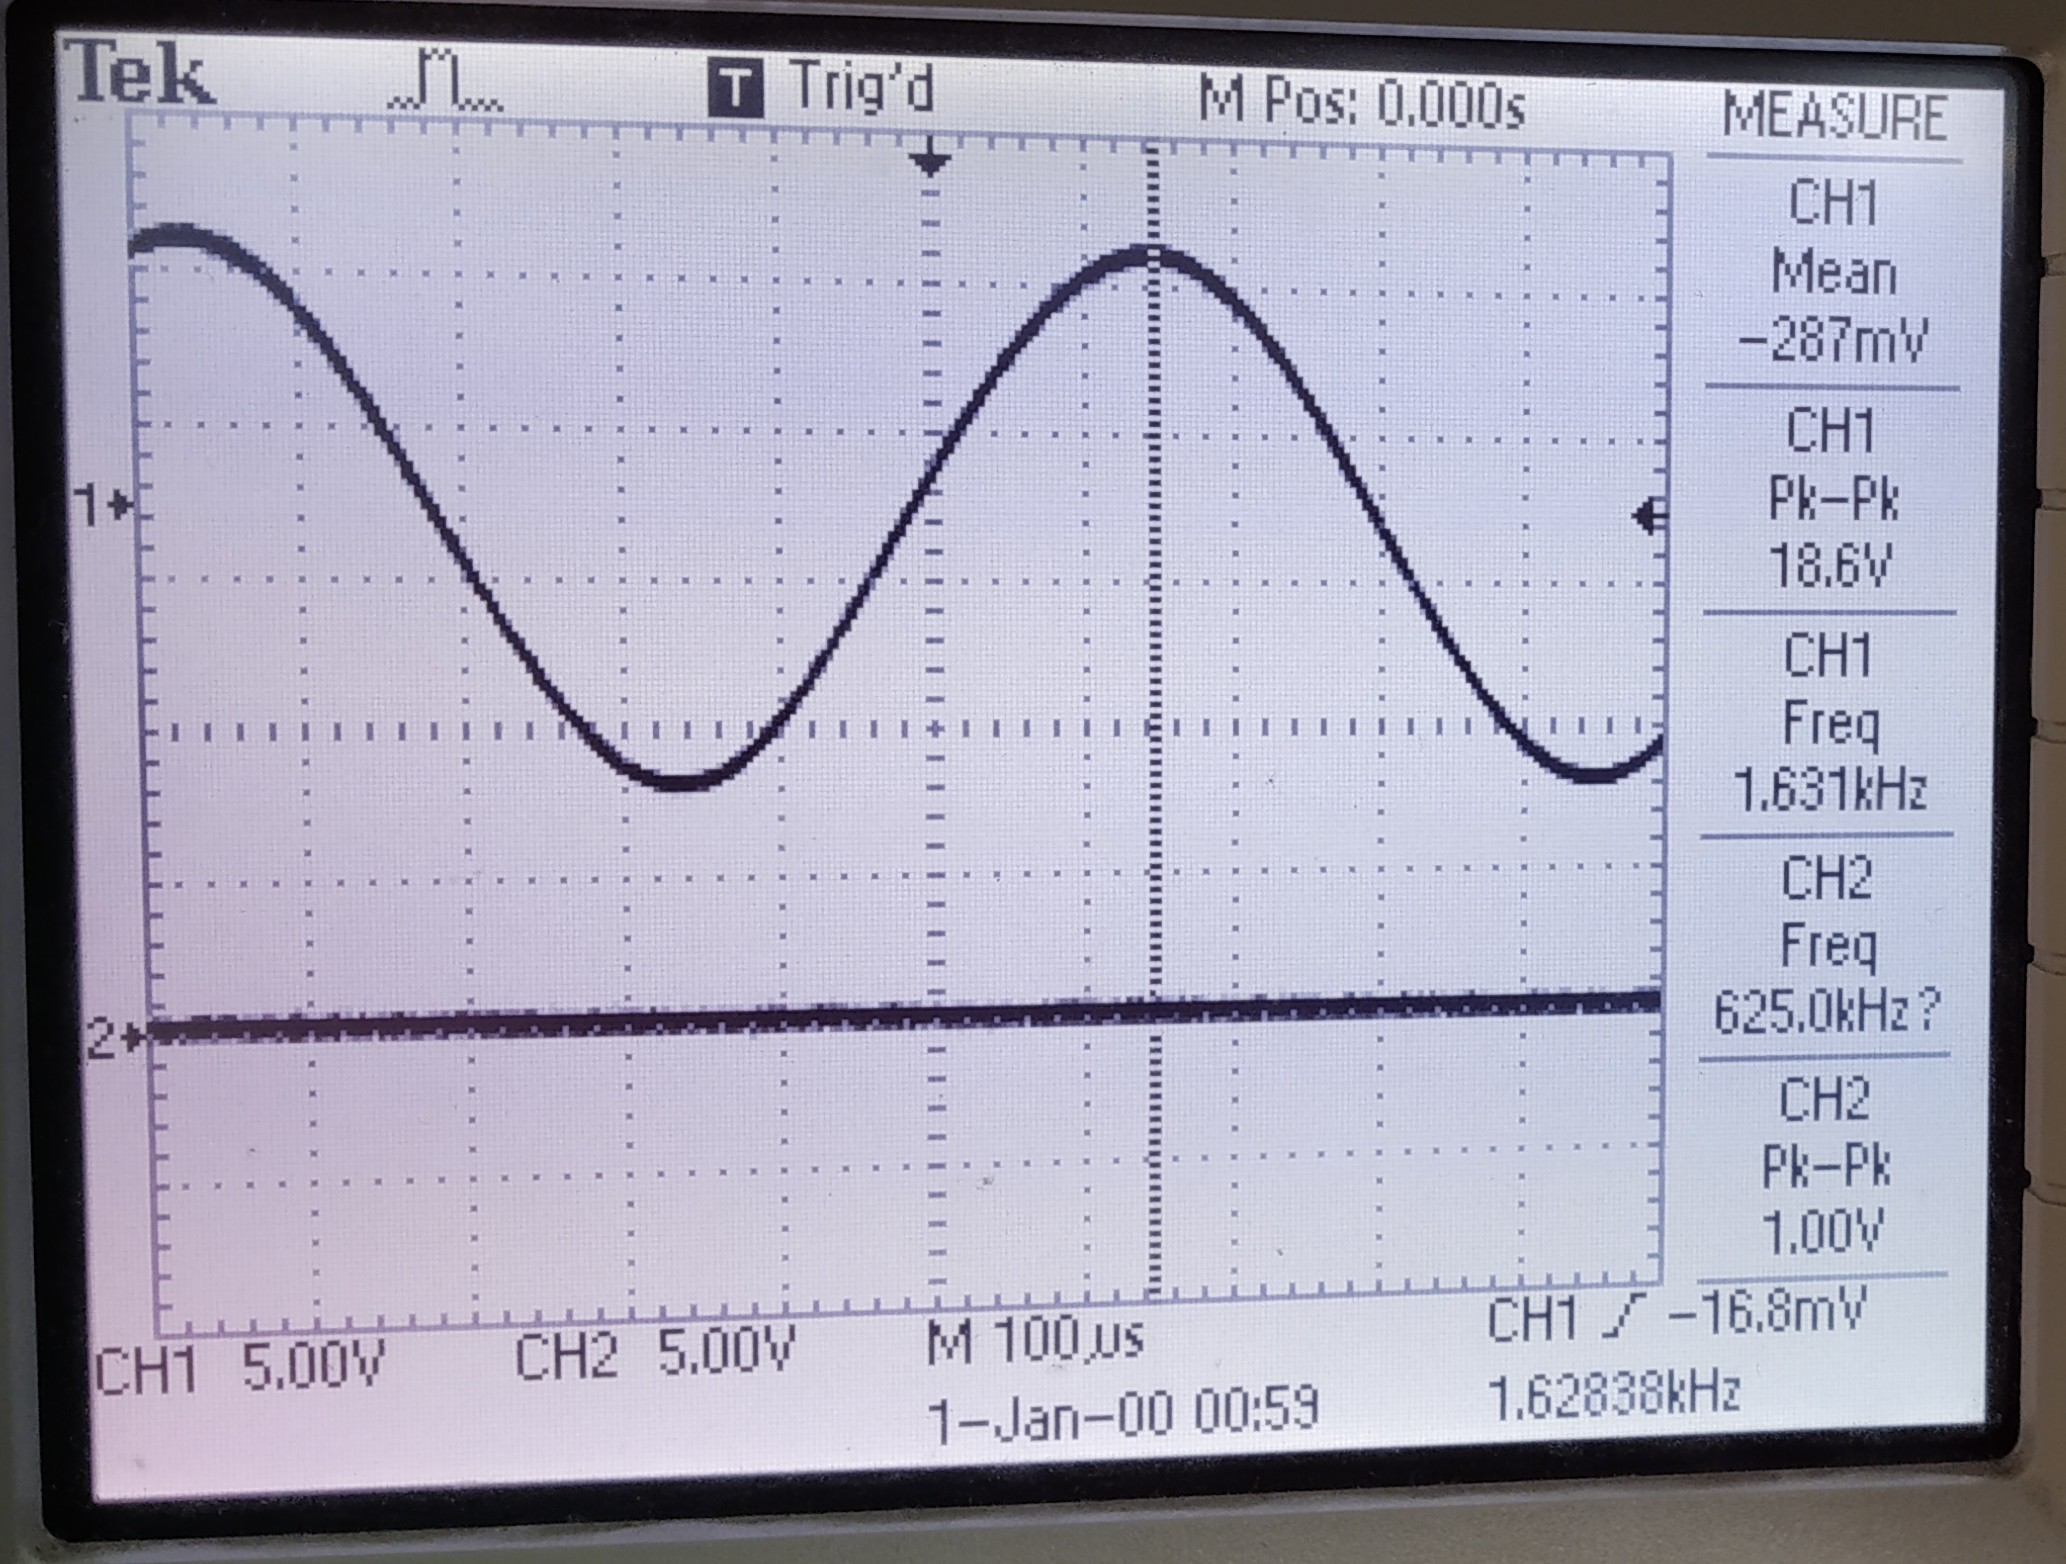
\includegraphics[width = 0.5\linewidth, height = 3in]{reports/lab5/wienBridge_stableOscillation.jpg}
            \caption{Wien Bridge stable oscillation waveform}
        \end{figure}
        \noindent
        The actual values of the resistances used are $R_1=9.78k\Omega$, $R_2=9.68k\Omega$, $R_3 = 9.79k\Omega$,  $R_4 = 9.74k\Omega$.\\\\
        Therefore, the approximate experimental frequency of oscillator is
        \begin{align}
            f &= \frac{1}{2\pi RC}\\
              &= \frac{1}{2\pi \times9.78k\times0.01\mu F}\\
              &= 1.627kHz
        \end{align}
        \noindent
        This almost matches the observed value i.e. 1.628kHz as can be seen in the above figure.
        % "Insert the peak to peak voltage and frequency value as seen in the DSO pic"
%%%%%%%%%%%%%%%%%%%%%%%%%%%%%%%%%%%%%%%%%%%%%%%%%%%%%%%%%%%%%%%%%%%%%%%%%%%%%%%%%%%%%%%%%%%%%%%%%%%%%%%%%%   
    \newpage
    \subsection{Wien Bridge Oscillator as voltage controlled oscillator}
        To make the Wien Bridge Oscillator work as voltage controlled oscillator, we design a circuit based on the op-amp TL084 and a LED-LDR pair as shown in fig. 13.
        % "Insert a pic of LED-LDR pair and of the circuit"
        \begin{figure}[H]
            \centering
            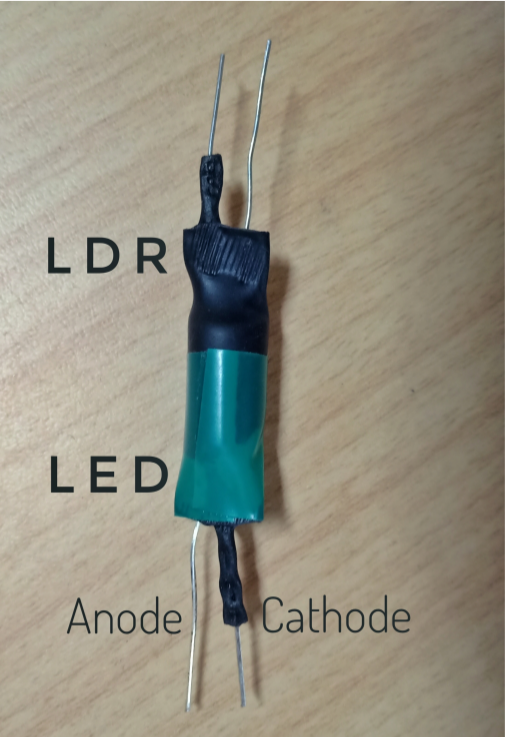
\includegraphics[width = 0.5\linewidth]{reports/lab5/ldr.png}
            \caption{LED-LDR pair}
        \end{figure}
        \noindent
        A photoresistor or LDR is an active component whose resistance decreases with respect to receiving luminosity on the component's sensitive surface. As, more current flows due to increase in input voltage, more illumination is observed in LED which in turn reduces the output resistance in non-linear fashion.\\\\ We plan to use this circuit for varying both $R_1$ and $R_2$ simultaneously (in the feedback network of the Wien Bridge Oscillator) in accordance with control voltage $V_C$, hence controlling its frequency as it is inversely proportional to resistances' value.\\

        \begin{figure}[H]
            \centering
            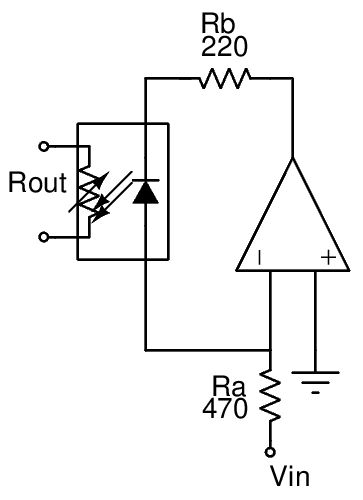
\includegraphics[width = 0.5\linewidth]{reports/lab5/p3.png}
            \caption{LED-LDR pair circuit for varying R_{out}}
        \end{figure}
        \noindent
        
        \noindent
        
        The graph of $R_{out} \text{ vs } V_{in}$ as we vary $V_{in}$ is plotted below:\\
        \begin{minipage}{\linewidth}
            \centering
            \begin{minipage}{0.4\linewidth}
                \begin{table}[H]
                    \centering
                    \begin{tabular}{|c|c|}\hline
                        $V_{in}(V)$ & $R_{out}(k\Omega)$\\\hline
                        0	&	96	\\	\hline
                        0.1	&	12.4	\\	\hline
                        0.2	&	6.6	\\	\hline
                        0.3	&	4.7	\\	\hline
                        0.5	&	3.0	\\	\hline
                        1.0	&	1.9	\\	\hline
                        1.5	&	1.6	\\	\hline
                        2.0	&	1.4	\\	\hline
                        2.5	&	1.2	\\	\hline
                        3.0	&	1.1	\\	\hline
                        3.5	&	1.1	\\	\hline
                
                    \end{tabular}
                    \caption{Observation Table}
                    \label{tab:my_label}
                \end{table}
            \end{minipage}
            \hspace{0.02\linewidth}
            \begin{minipage}{0.56\linewidth}
                \begin{figure}[H]
                    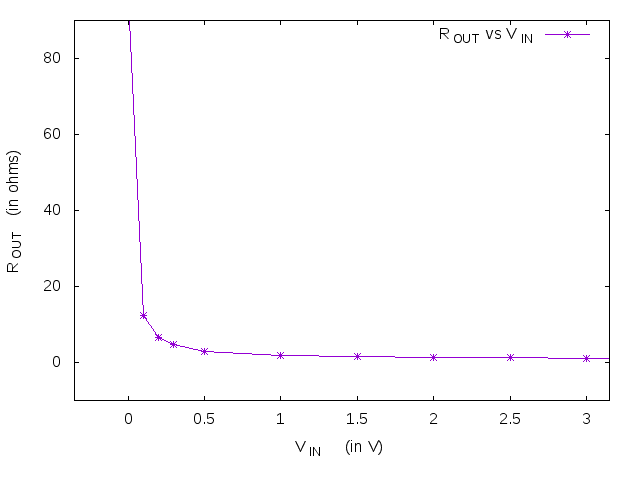
\includegraphics[width=\linewidth]{reports/lab5/rout.png}
                    \caption{Variation of R_{out} with change in V_{IN}}
                    \label{Va_0_yt}
                \end{figure}
            \end{minipage}
        \end{minipage}
    %%%%%%%%%%%%%%%%%%%%%%%%%%%%%%%%%%%%%%%%%%%%%%%%%%%%%%%%%%%%%%%%%%%%%%%%%%%%%%%%%%%%%%%%%%%%%%%%%%%%%    
    \subsection{Sweep Generator}
    
        Here, finally we combine the circuits of wien bridge oscillator and the LED-LDR to get the desired sine sweep generator.\\\\
        \noindent
        Since the two LED's are connected in series, the current flowing through them will be the same. Now as $V_{in}$ increases, both $R_1$ and $R_2$ decrease such that the magnitude of both are equal to each other. As $R_1$ and $R_2$ decrease, the frequency of the Wien Bridge Oscillator increases. \\\\
        \noindent
        The final circuit is as shown below, we use here 3 LED-LDR pair circuits. Two of these circuits are for varying the resistors present in the feedback network of the oscillator. The third circuit is used because as the frequency changes, the amplitude of the output waveform is likely to decrease, so we vary this third additional resistor to increase the gain and maintain a fixed amplitude of the output. 
        \begin{figure}[H]
            \centering
            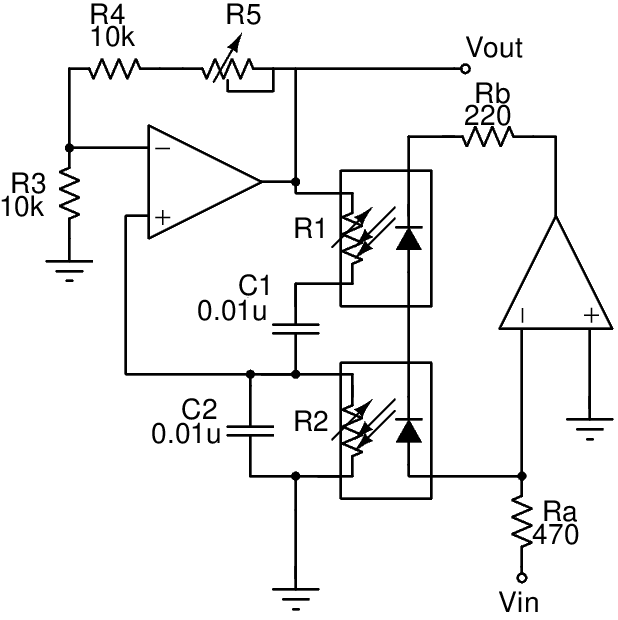
\includegraphics[width = 0.5\linewidth]{reports/lab5/p4.png}
            \caption{Sweep Generator}
        \end{figure}
        \noindent
        To verify whether our proposed circuit changes frequency on varying the input voltage, we note the waveform for $V_c = 0V$, $0.5V$, $1V$, and $1.5V$.
        \begin{figure}[H]
            \centering
            \begin{subfigure}{.5\textwidth}
                \centering
                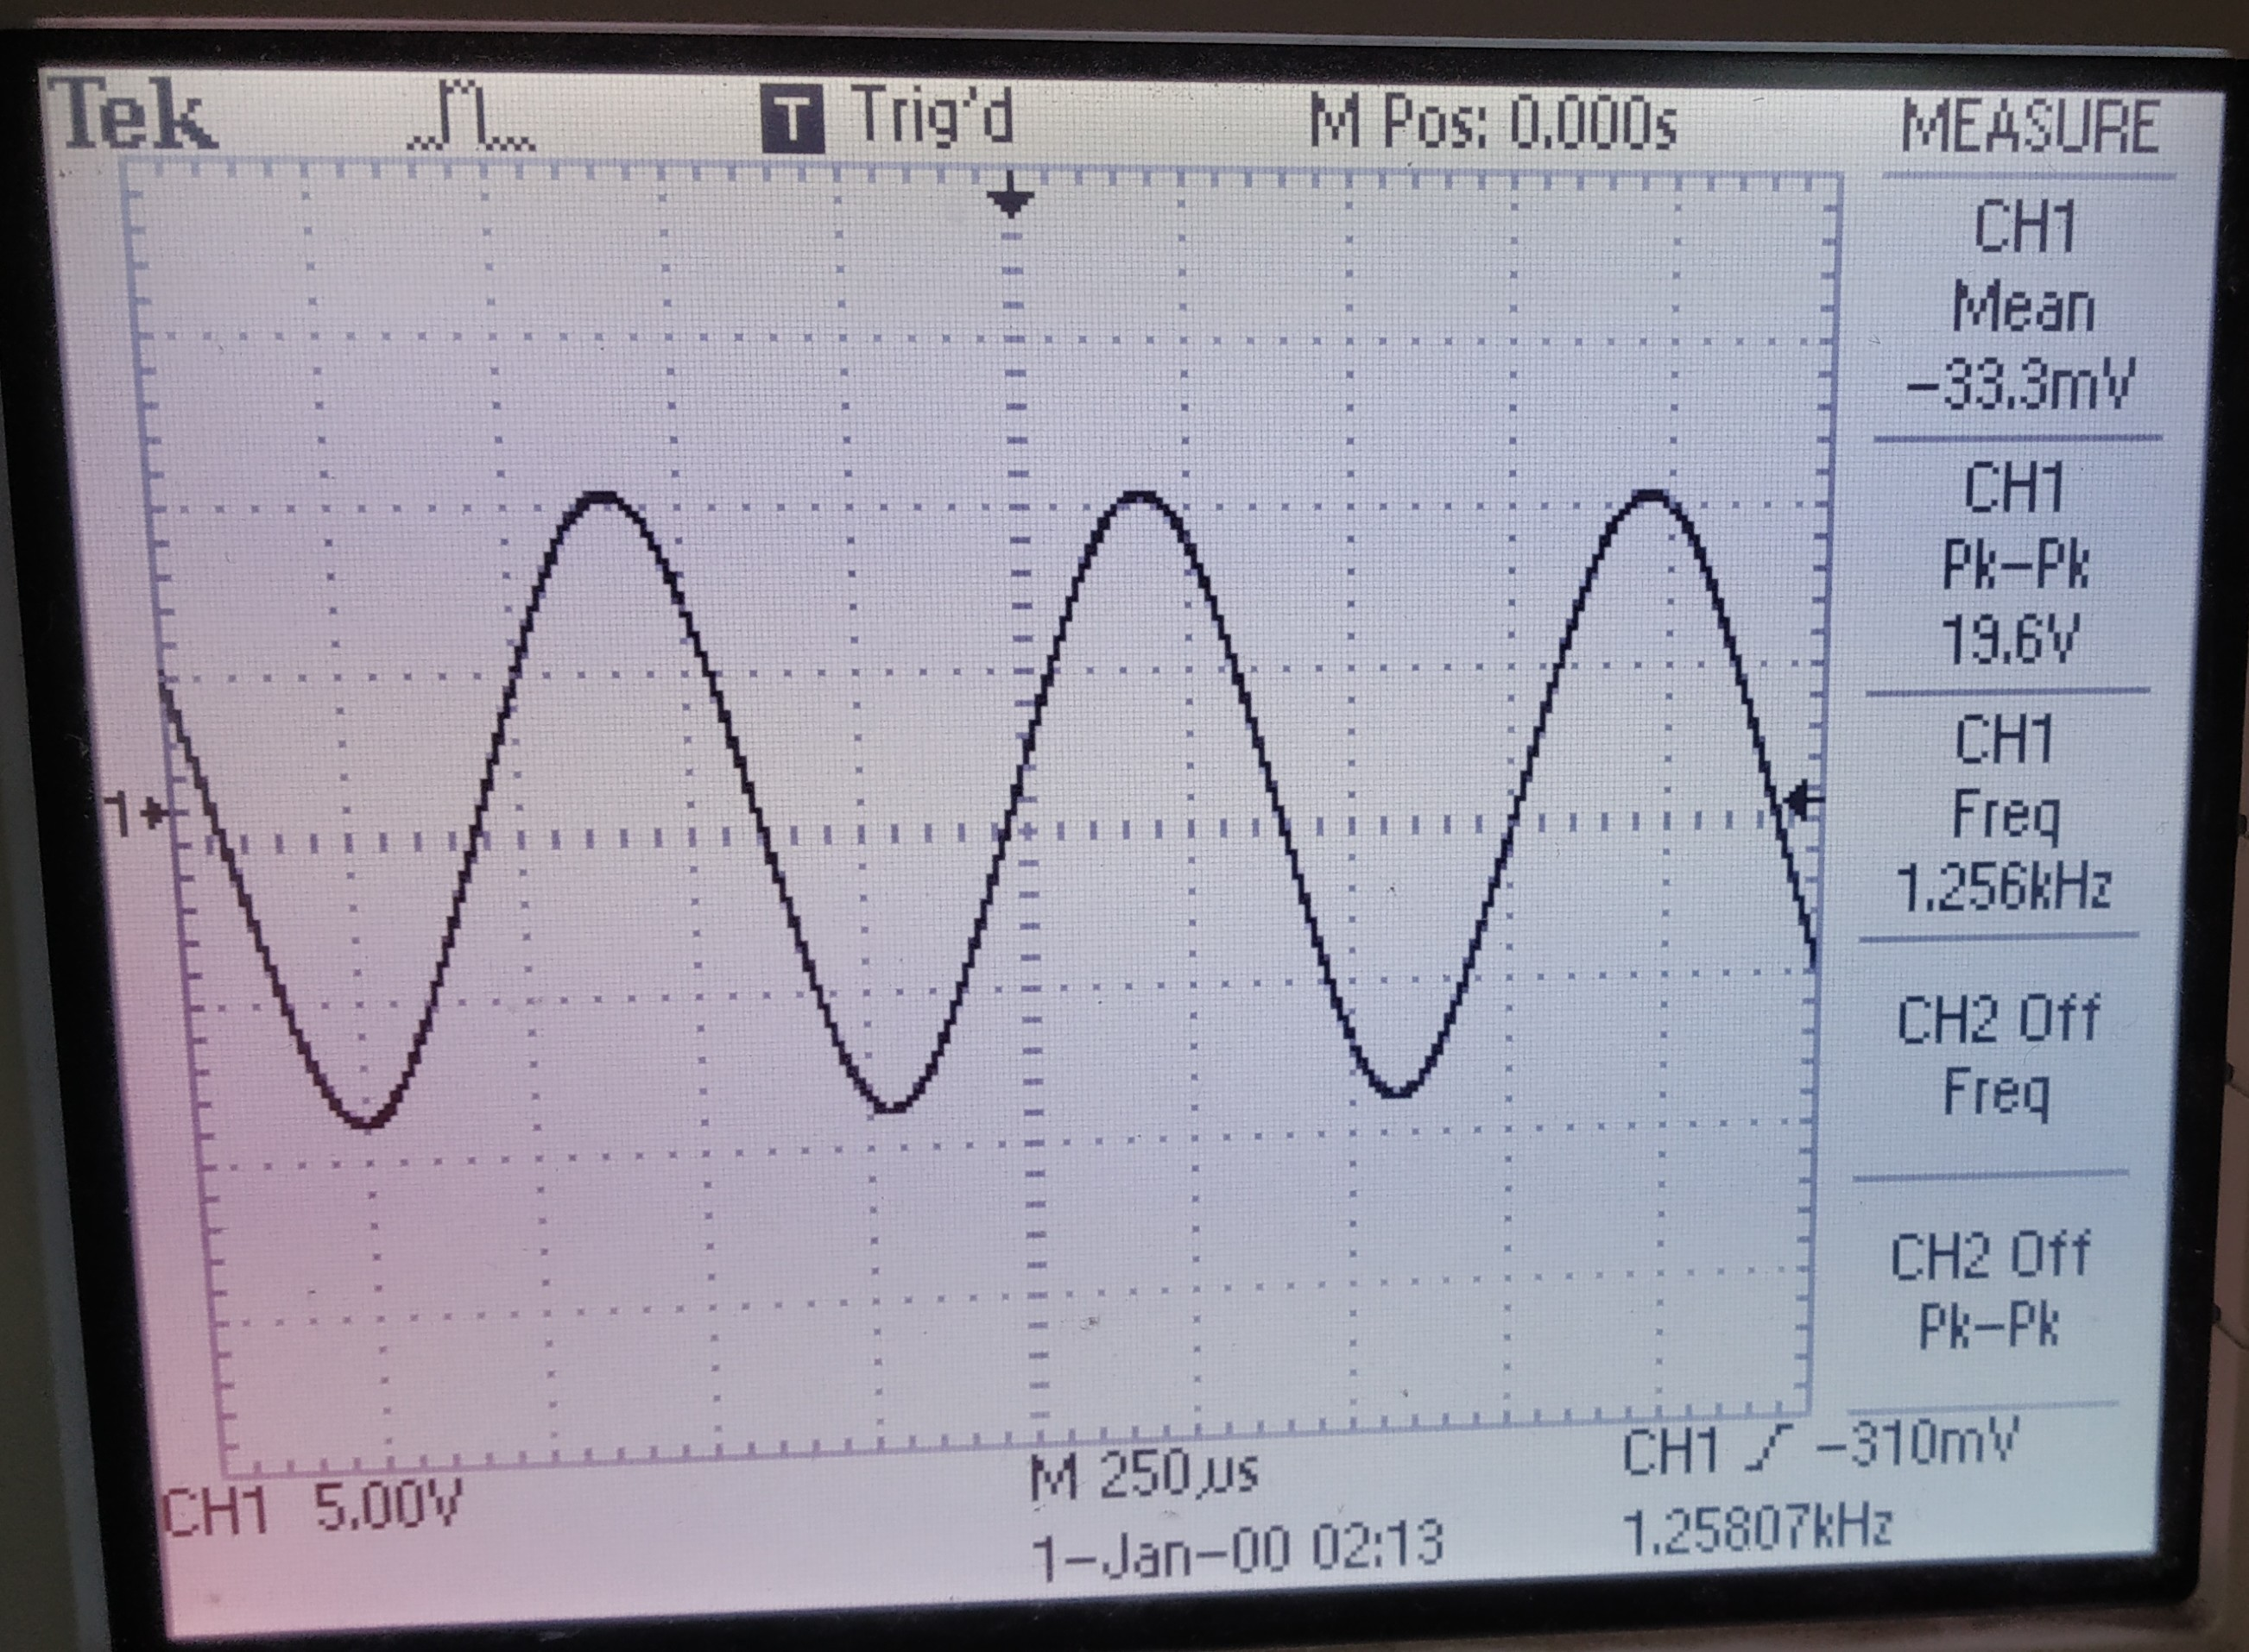
\includegraphics[width=70mm]{reports/lab5/Vc_0V.jpg}
                \caption{V_C = 0V}
            \end{subfigure}%
            \begin{subfigure}{.5\textwidth}
                \centering
                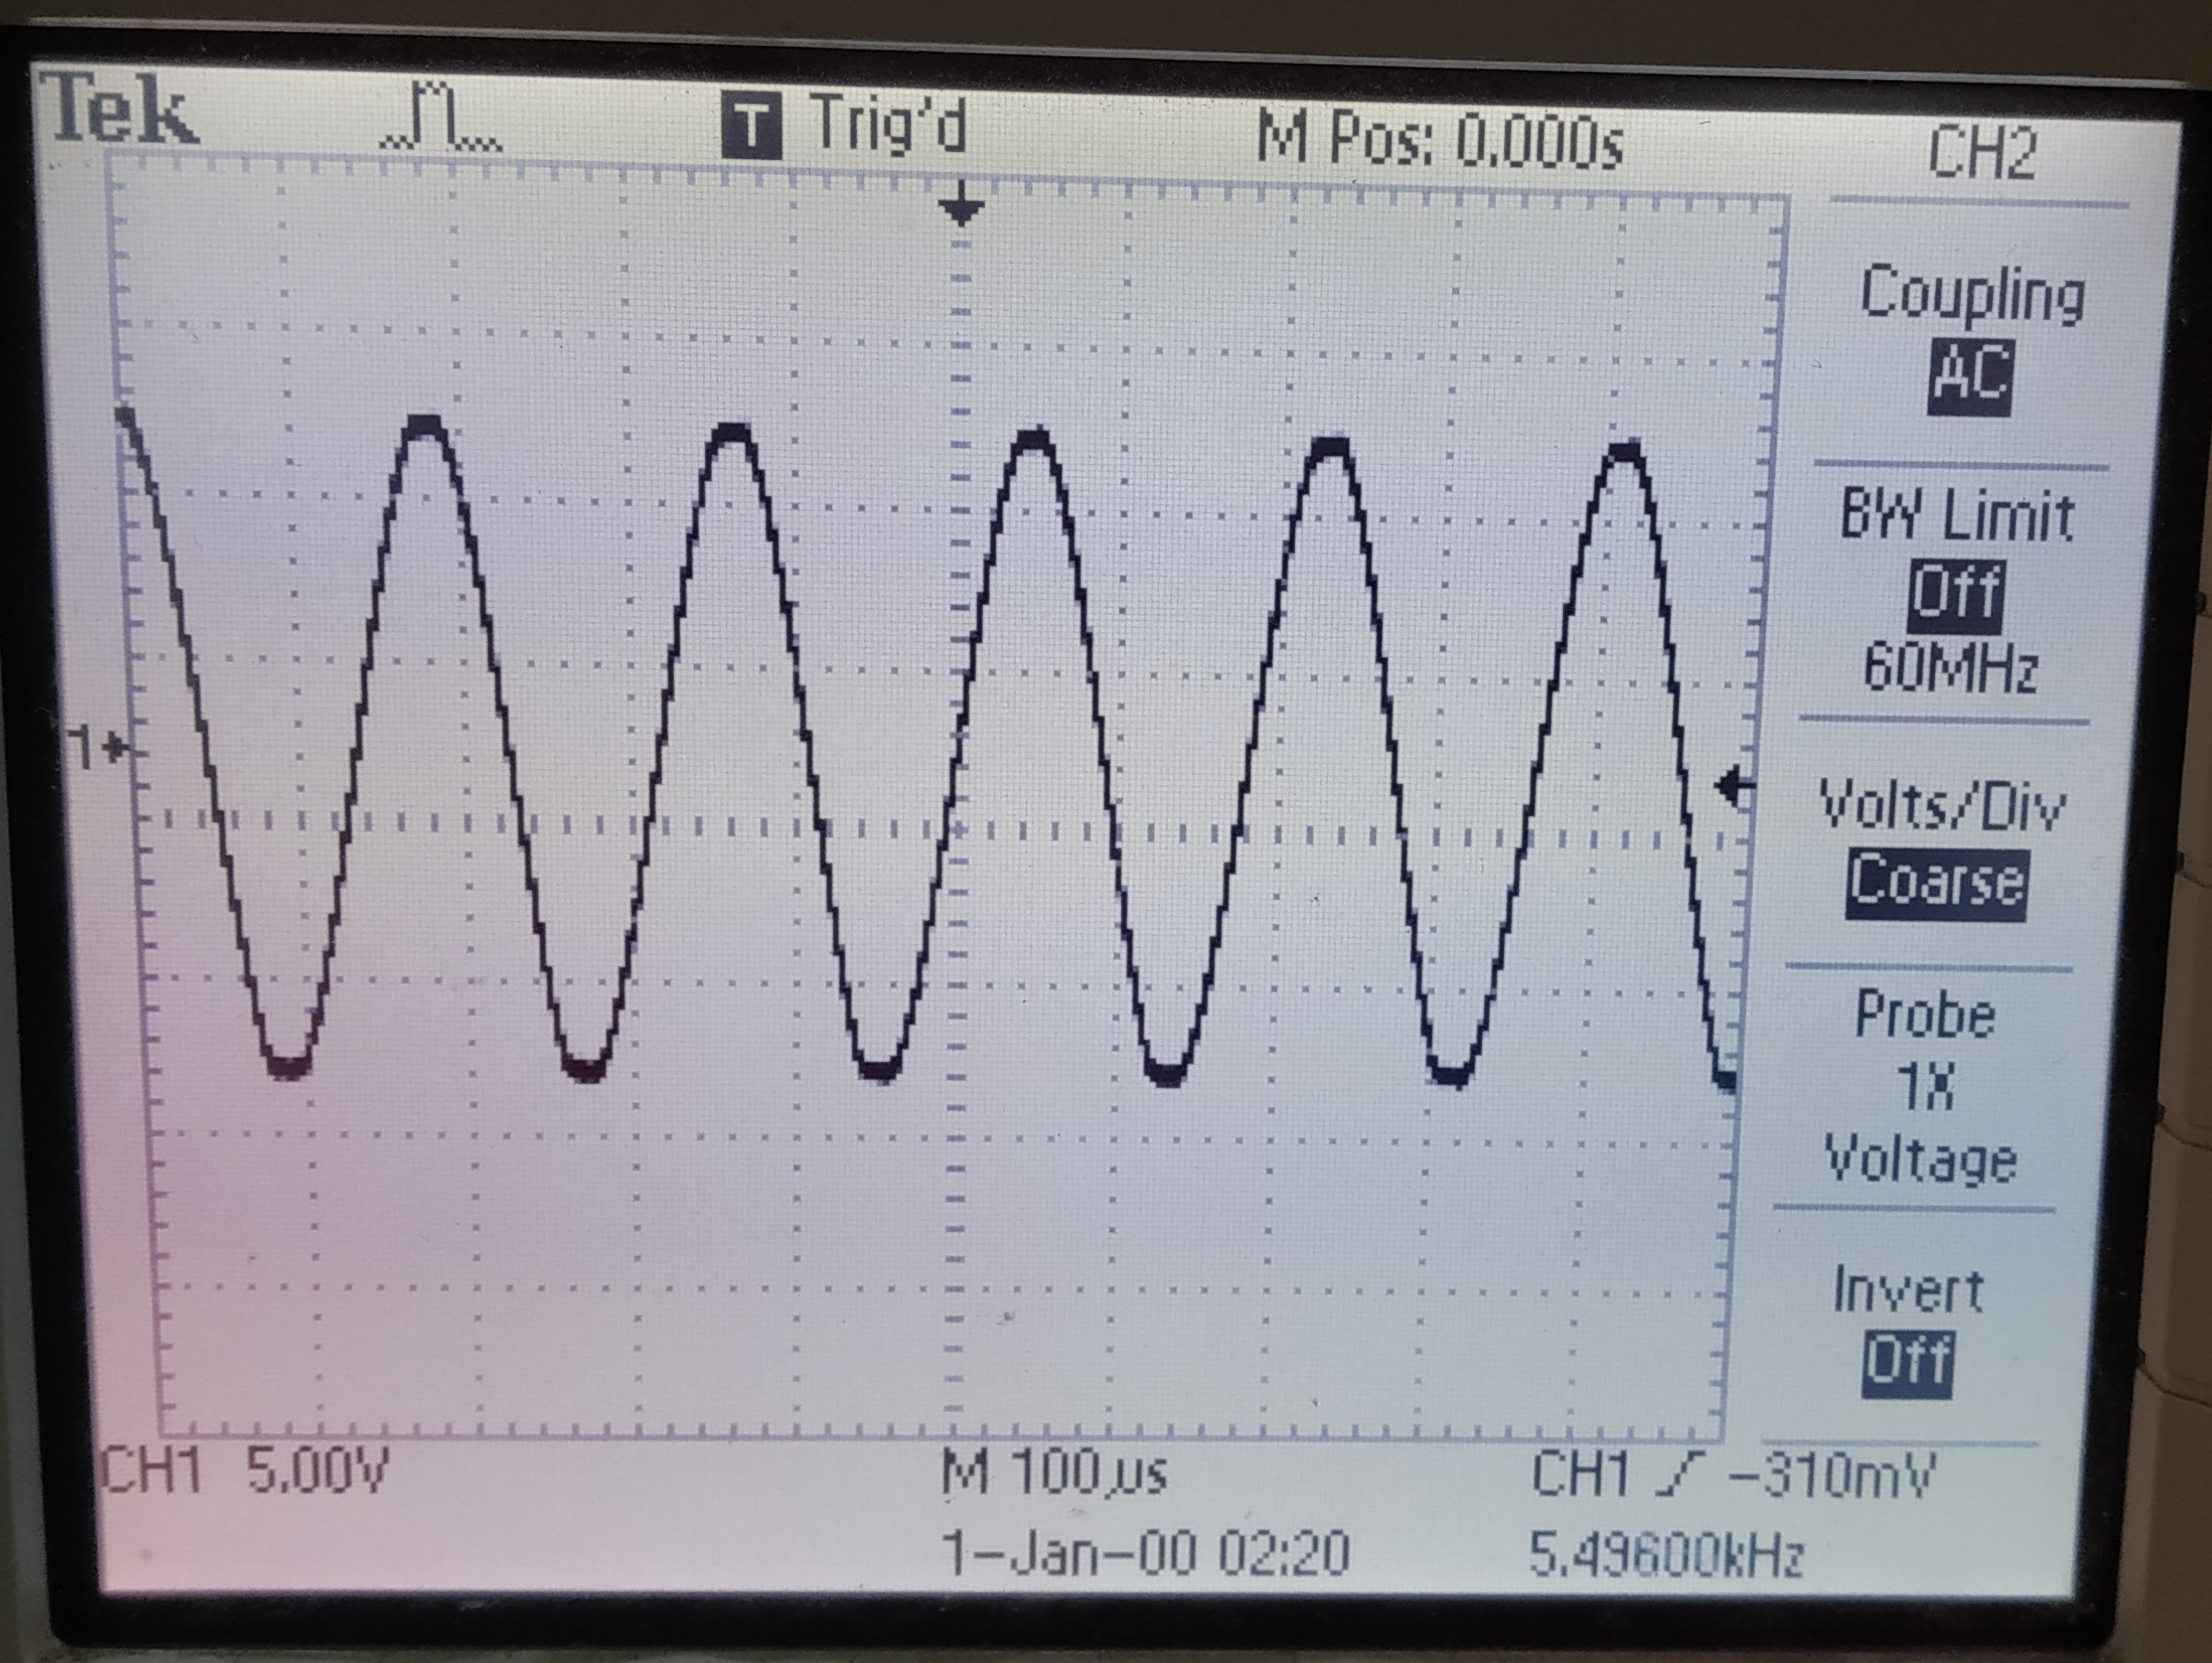
\includegraphics[width=70mm]{reports/lab5/Vc_0_5V.jpg}
                \caption{$V_C = 0.5V$}
            \end{subfigure}%
        \end{figure}
        \begin{figure}[H]
            \centering
            \begin{subfigure}{.5\textwidth}
                \centering
                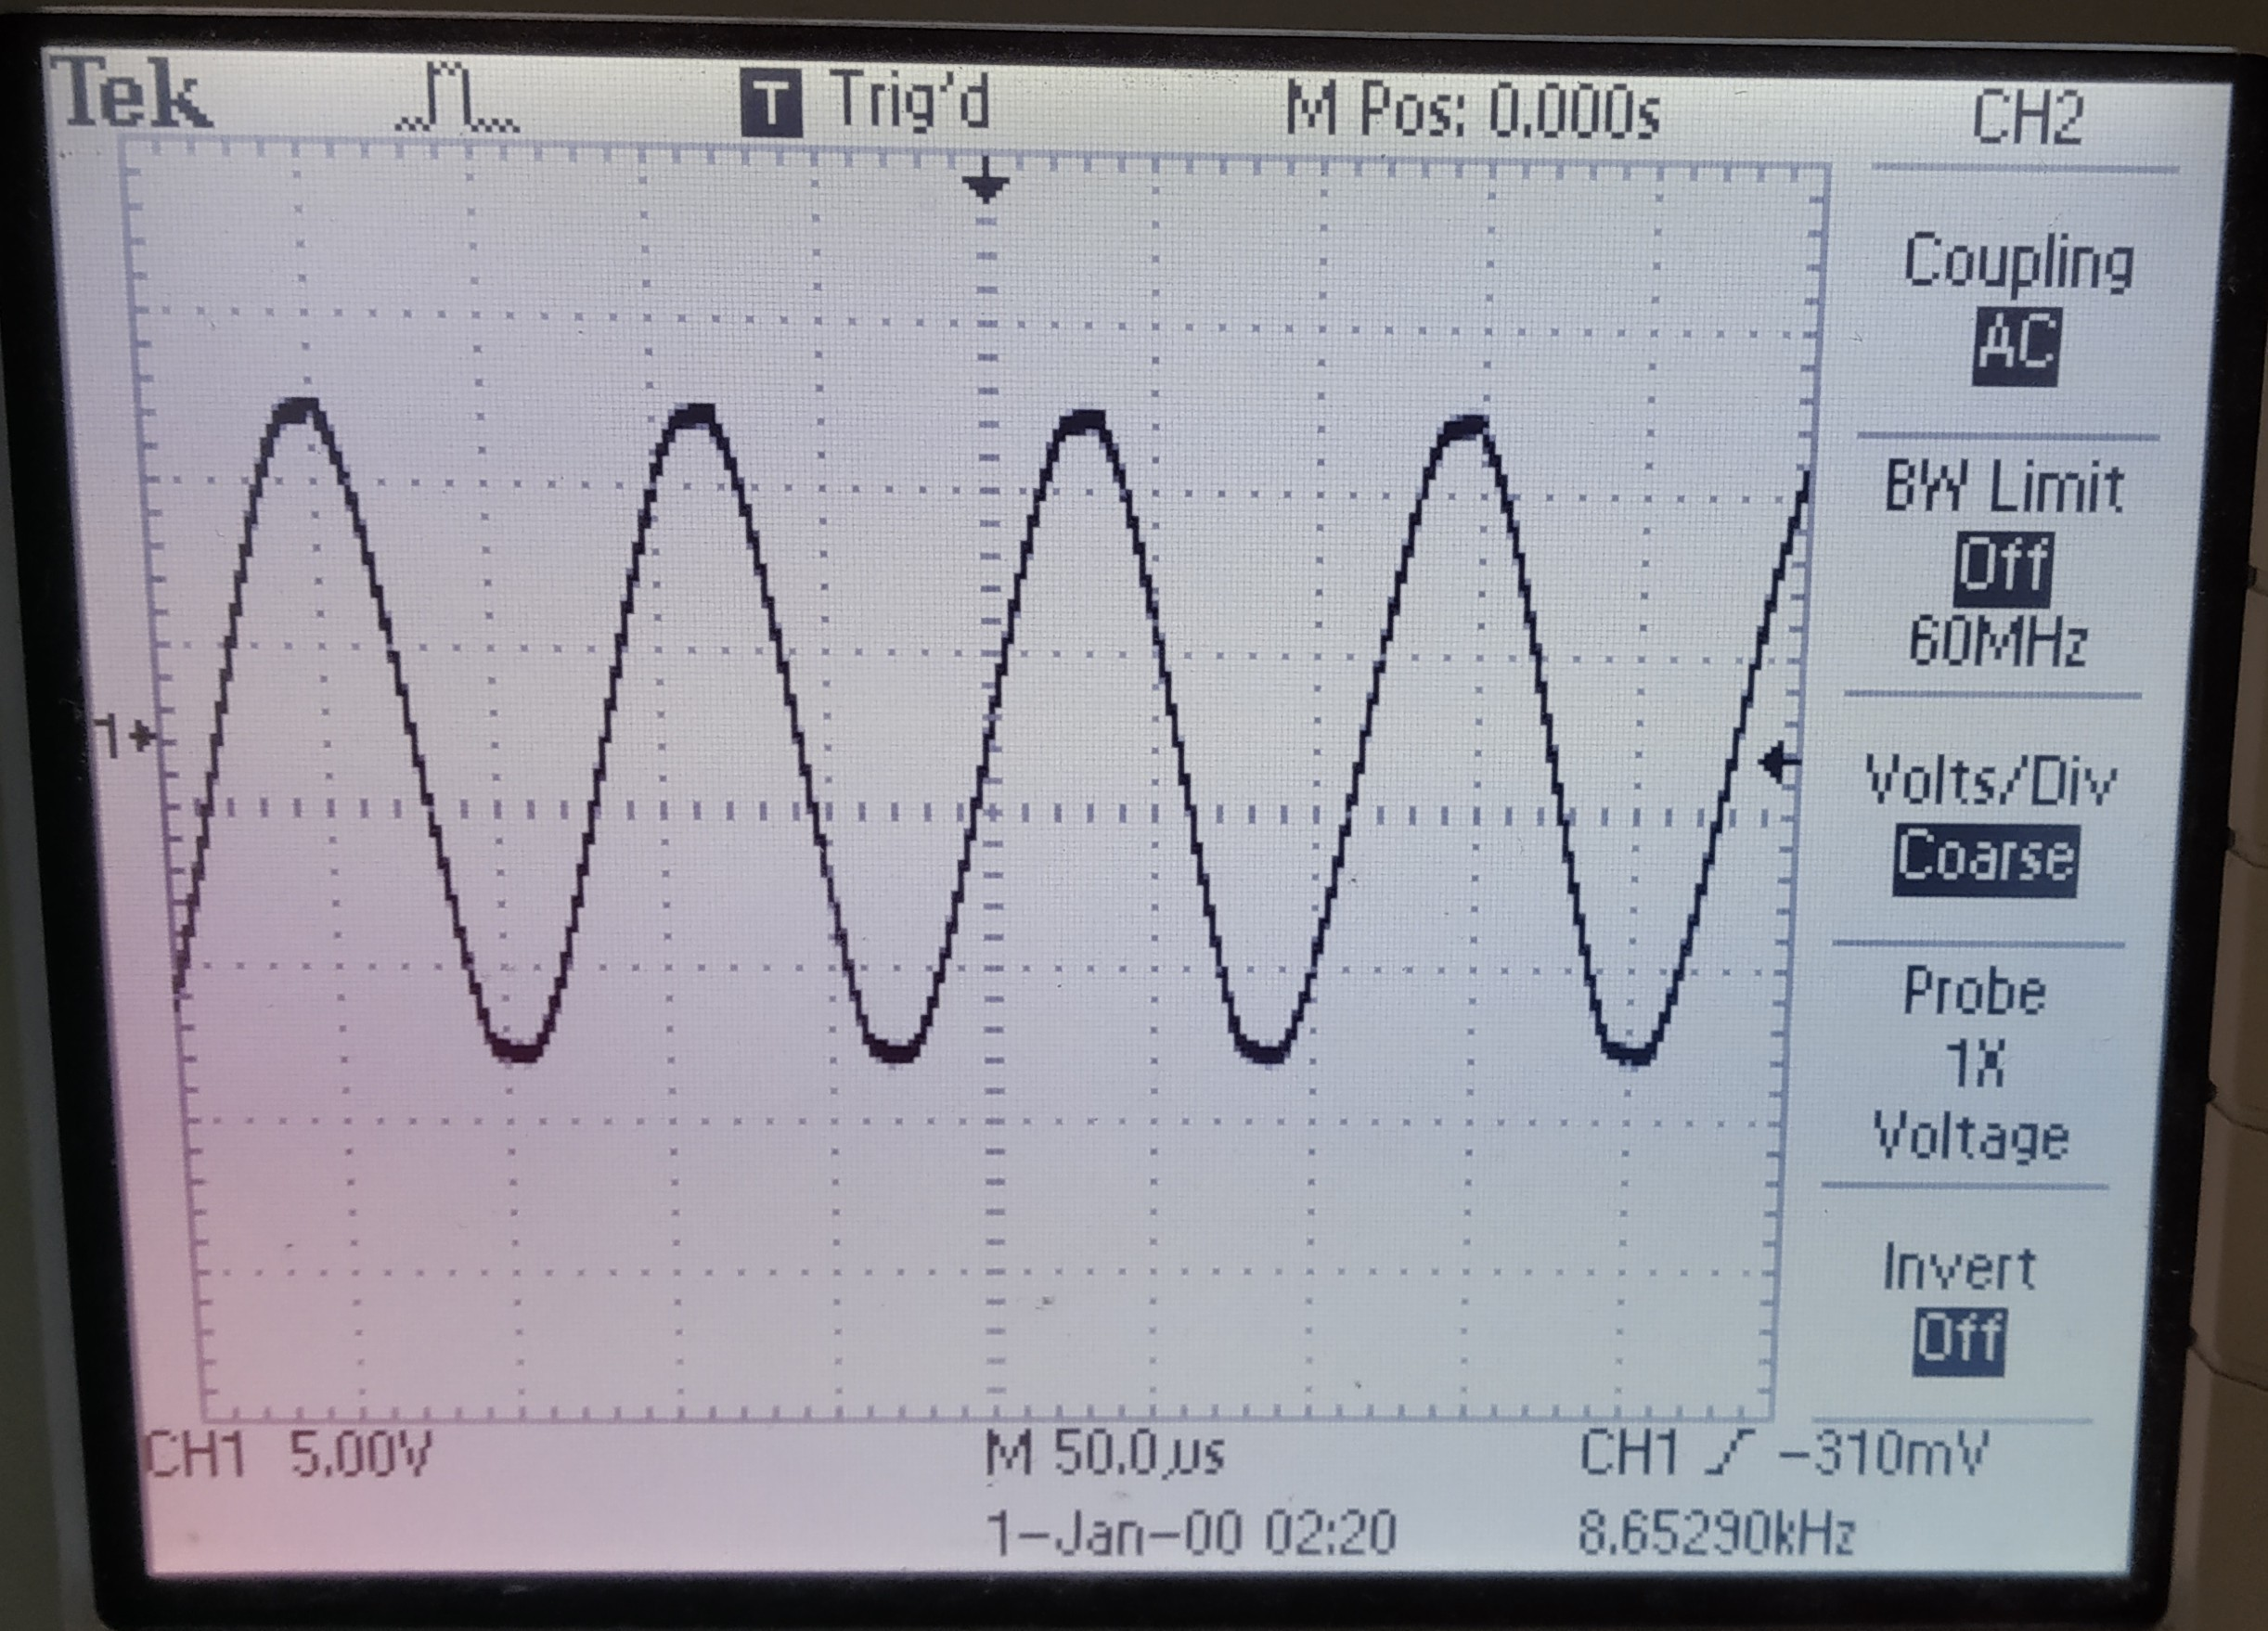
\includegraphics[width=70mm]{reports/lab5/Vc_1V.jpg}
                \caption{V_C = 1V}
            \end{subfigure}%
            \begin{subfigure}{.5\textwidth}
                \centering
                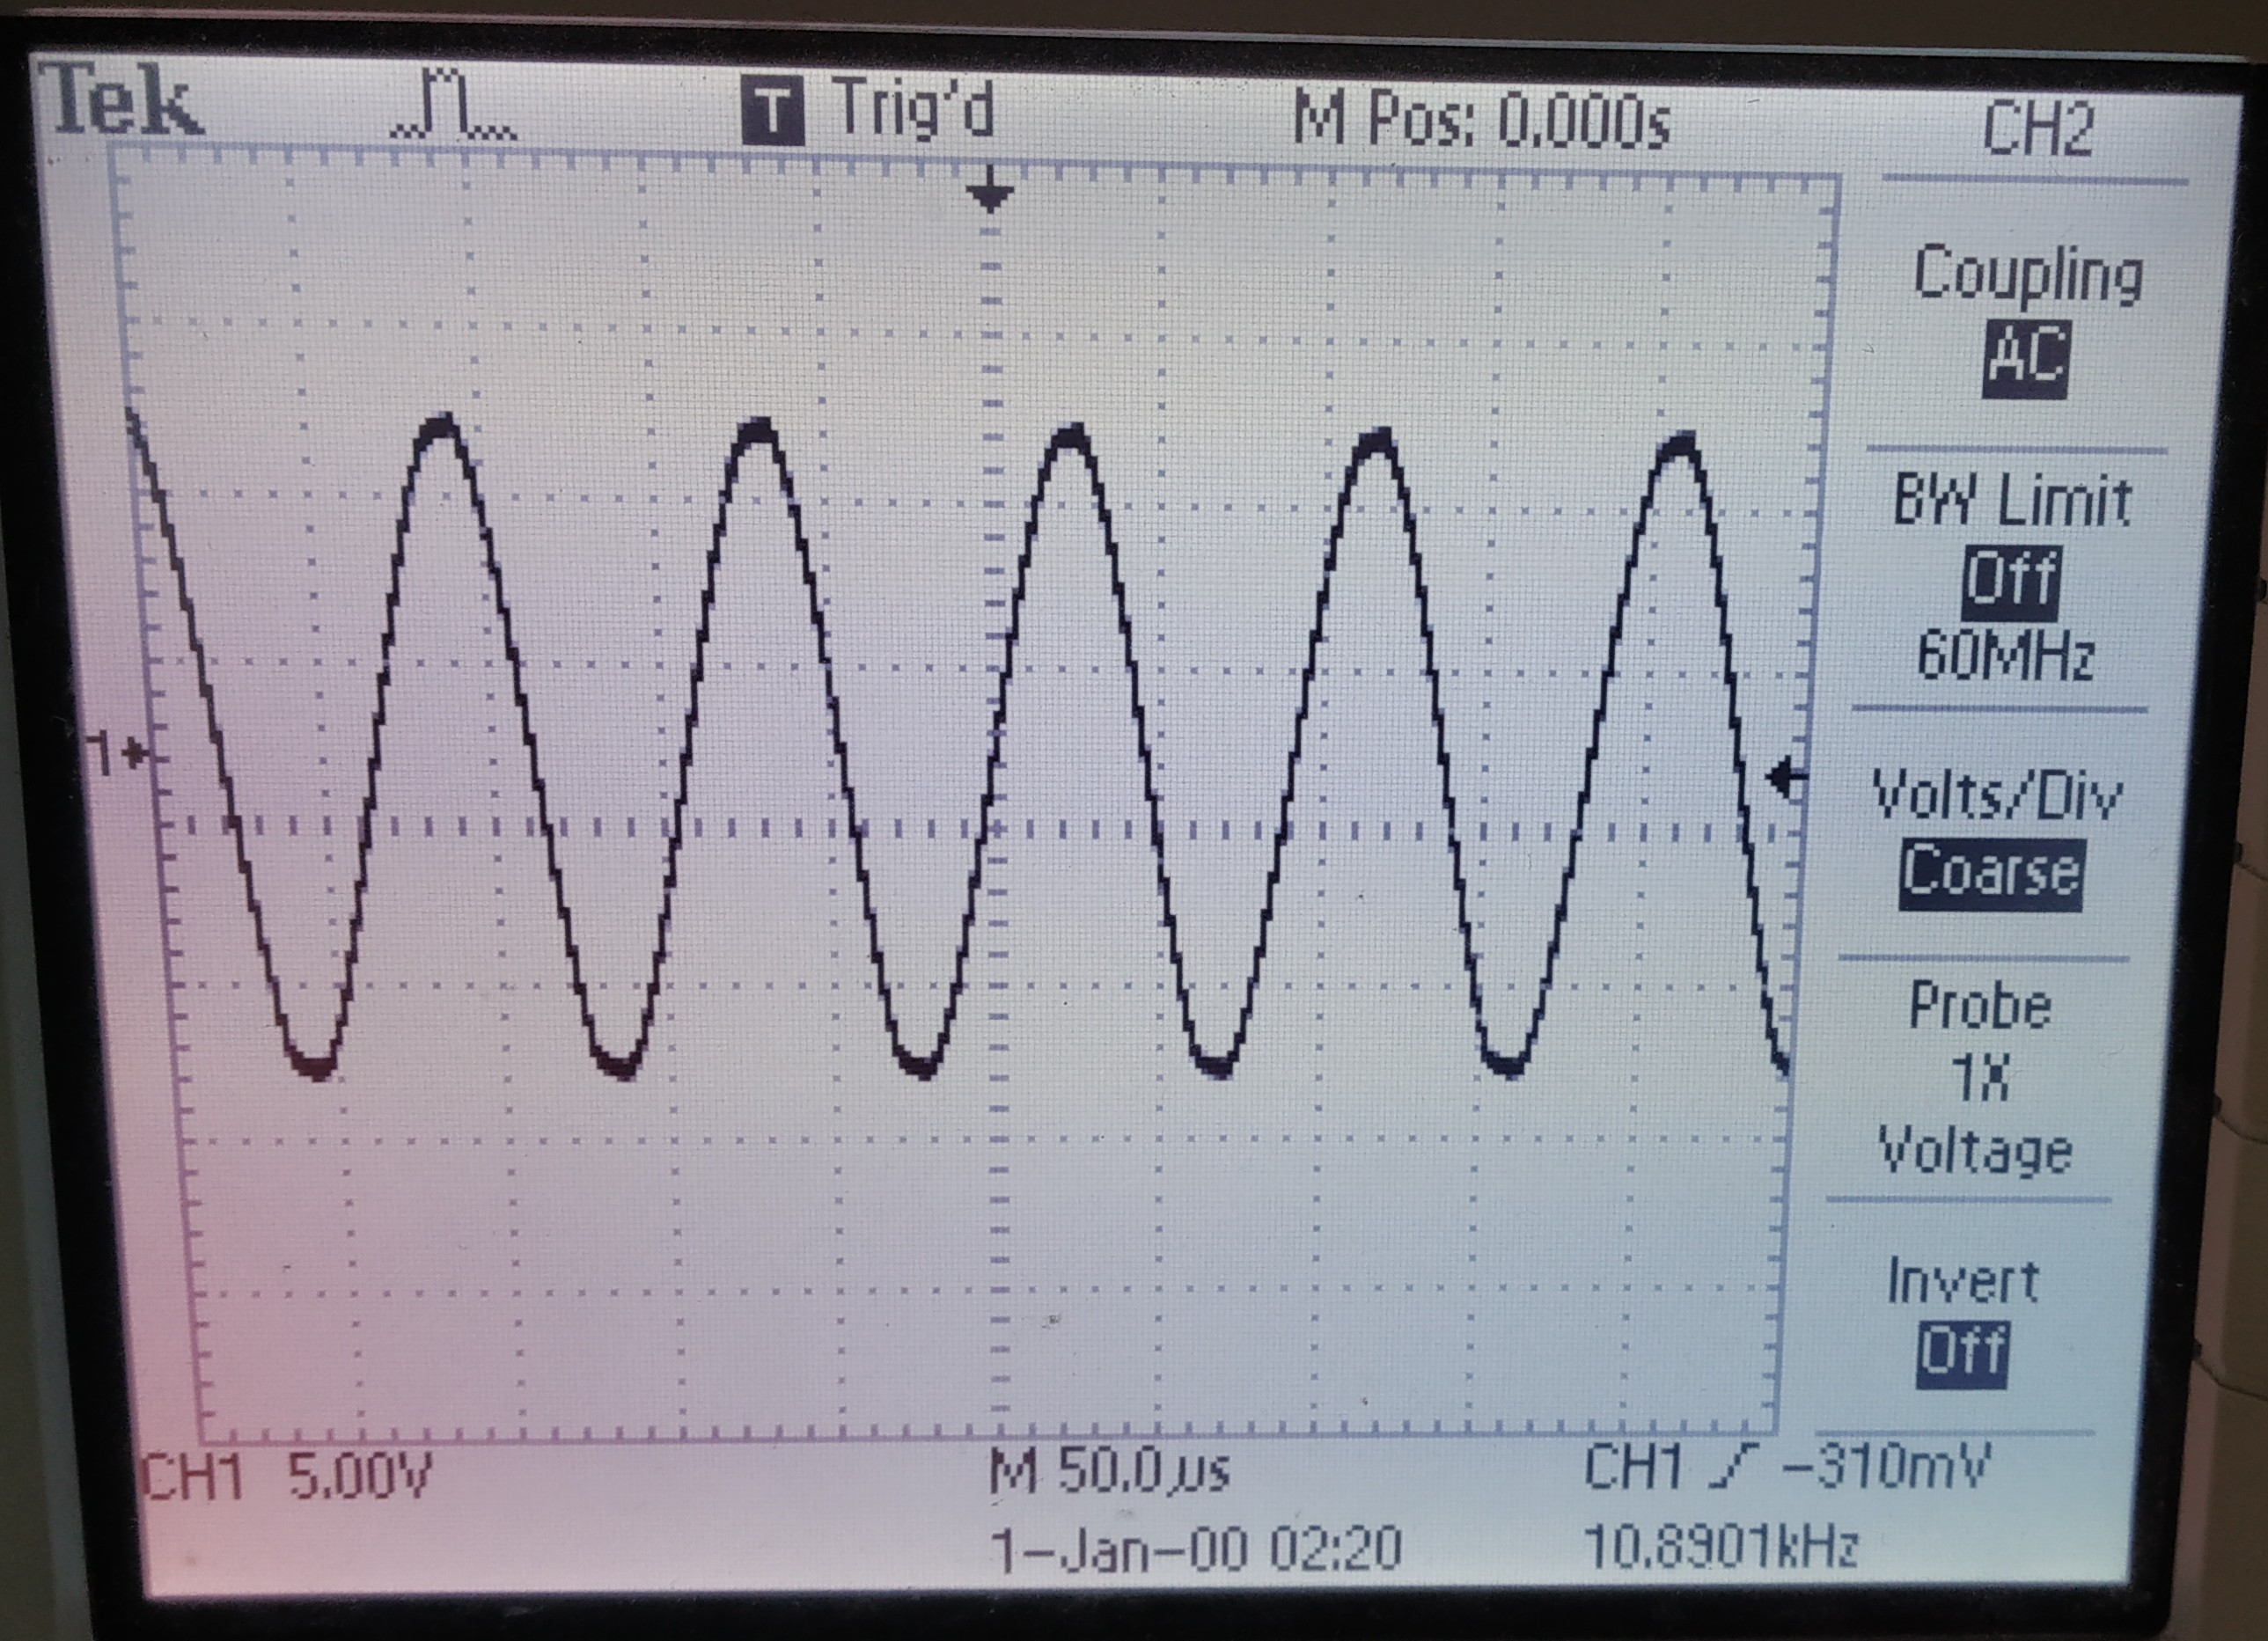
\includegraphics[width=70mm]{reports/lab5/Vc_1_5V.jpg}
                \caption{V_C = 1.5V}
            \end{subfigure}%
        \end{figure}
        
        % "Insert conclusion and a question is to be answered"

    \subsection{Sweep Generator and High Pass Filter}
        The circuit of Sallen Key High pass filter is shown below.
        \begin{figure}[H]
            \centering
            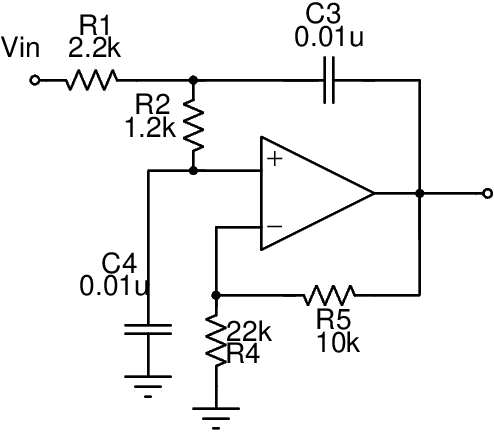
\includegraphics[width = 0.4\linewidth]{reports/lab5/p6.png}
            \caption{High Pass Filter}
        \end{figure}
        \noindent
        The maximum and minimum frequencies obtained at the output of the Sweep Generator was 3kHz and 10.3kHz
        \\\\
        The final circuit joining the sweep generator with the high pass filter is shown below.
        \begin{figure}[H]
            \centering
            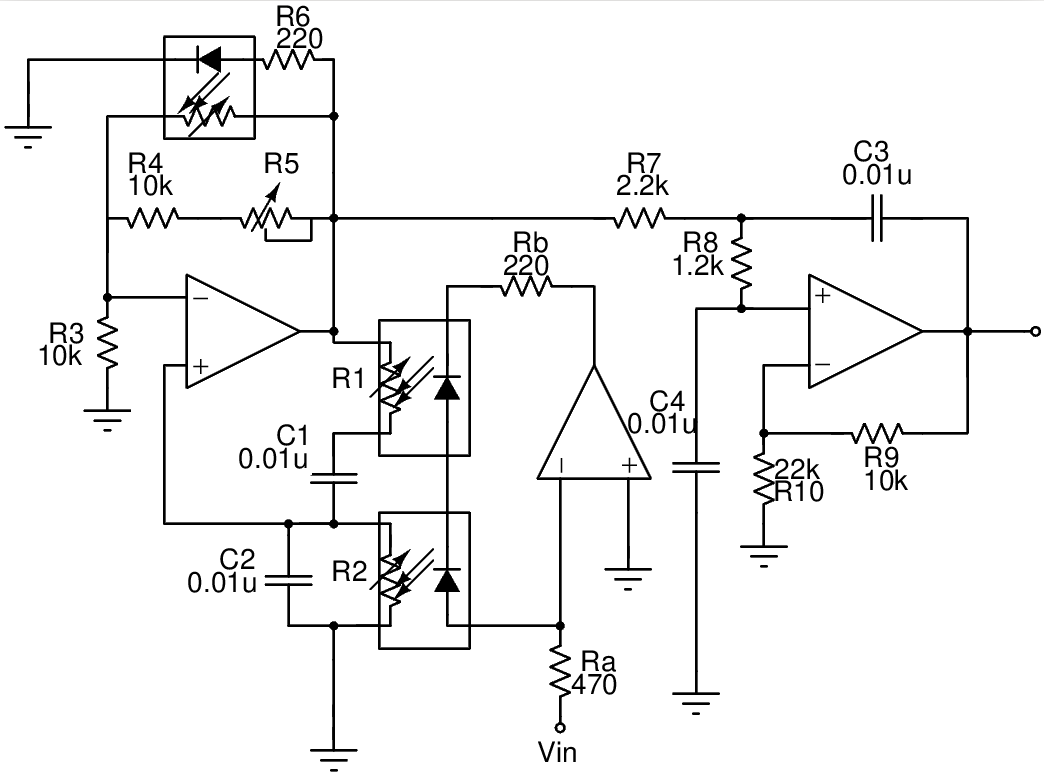
\includegraphics[width = 0.6\linewidth]{reports/lab5/p7.png}
            \caption{Sweep generator with High Pass Filter}
        \end{figure}
        \noindent
        The output waveform obtained on DSO, on connecting our sine sweep generator to the input of a second order Sallen Key High pass filter is shown below:\\\\
        \begin{figure}[H]
            \centering
            \begin{subfigure}{.5\textwidth}
                \centering
                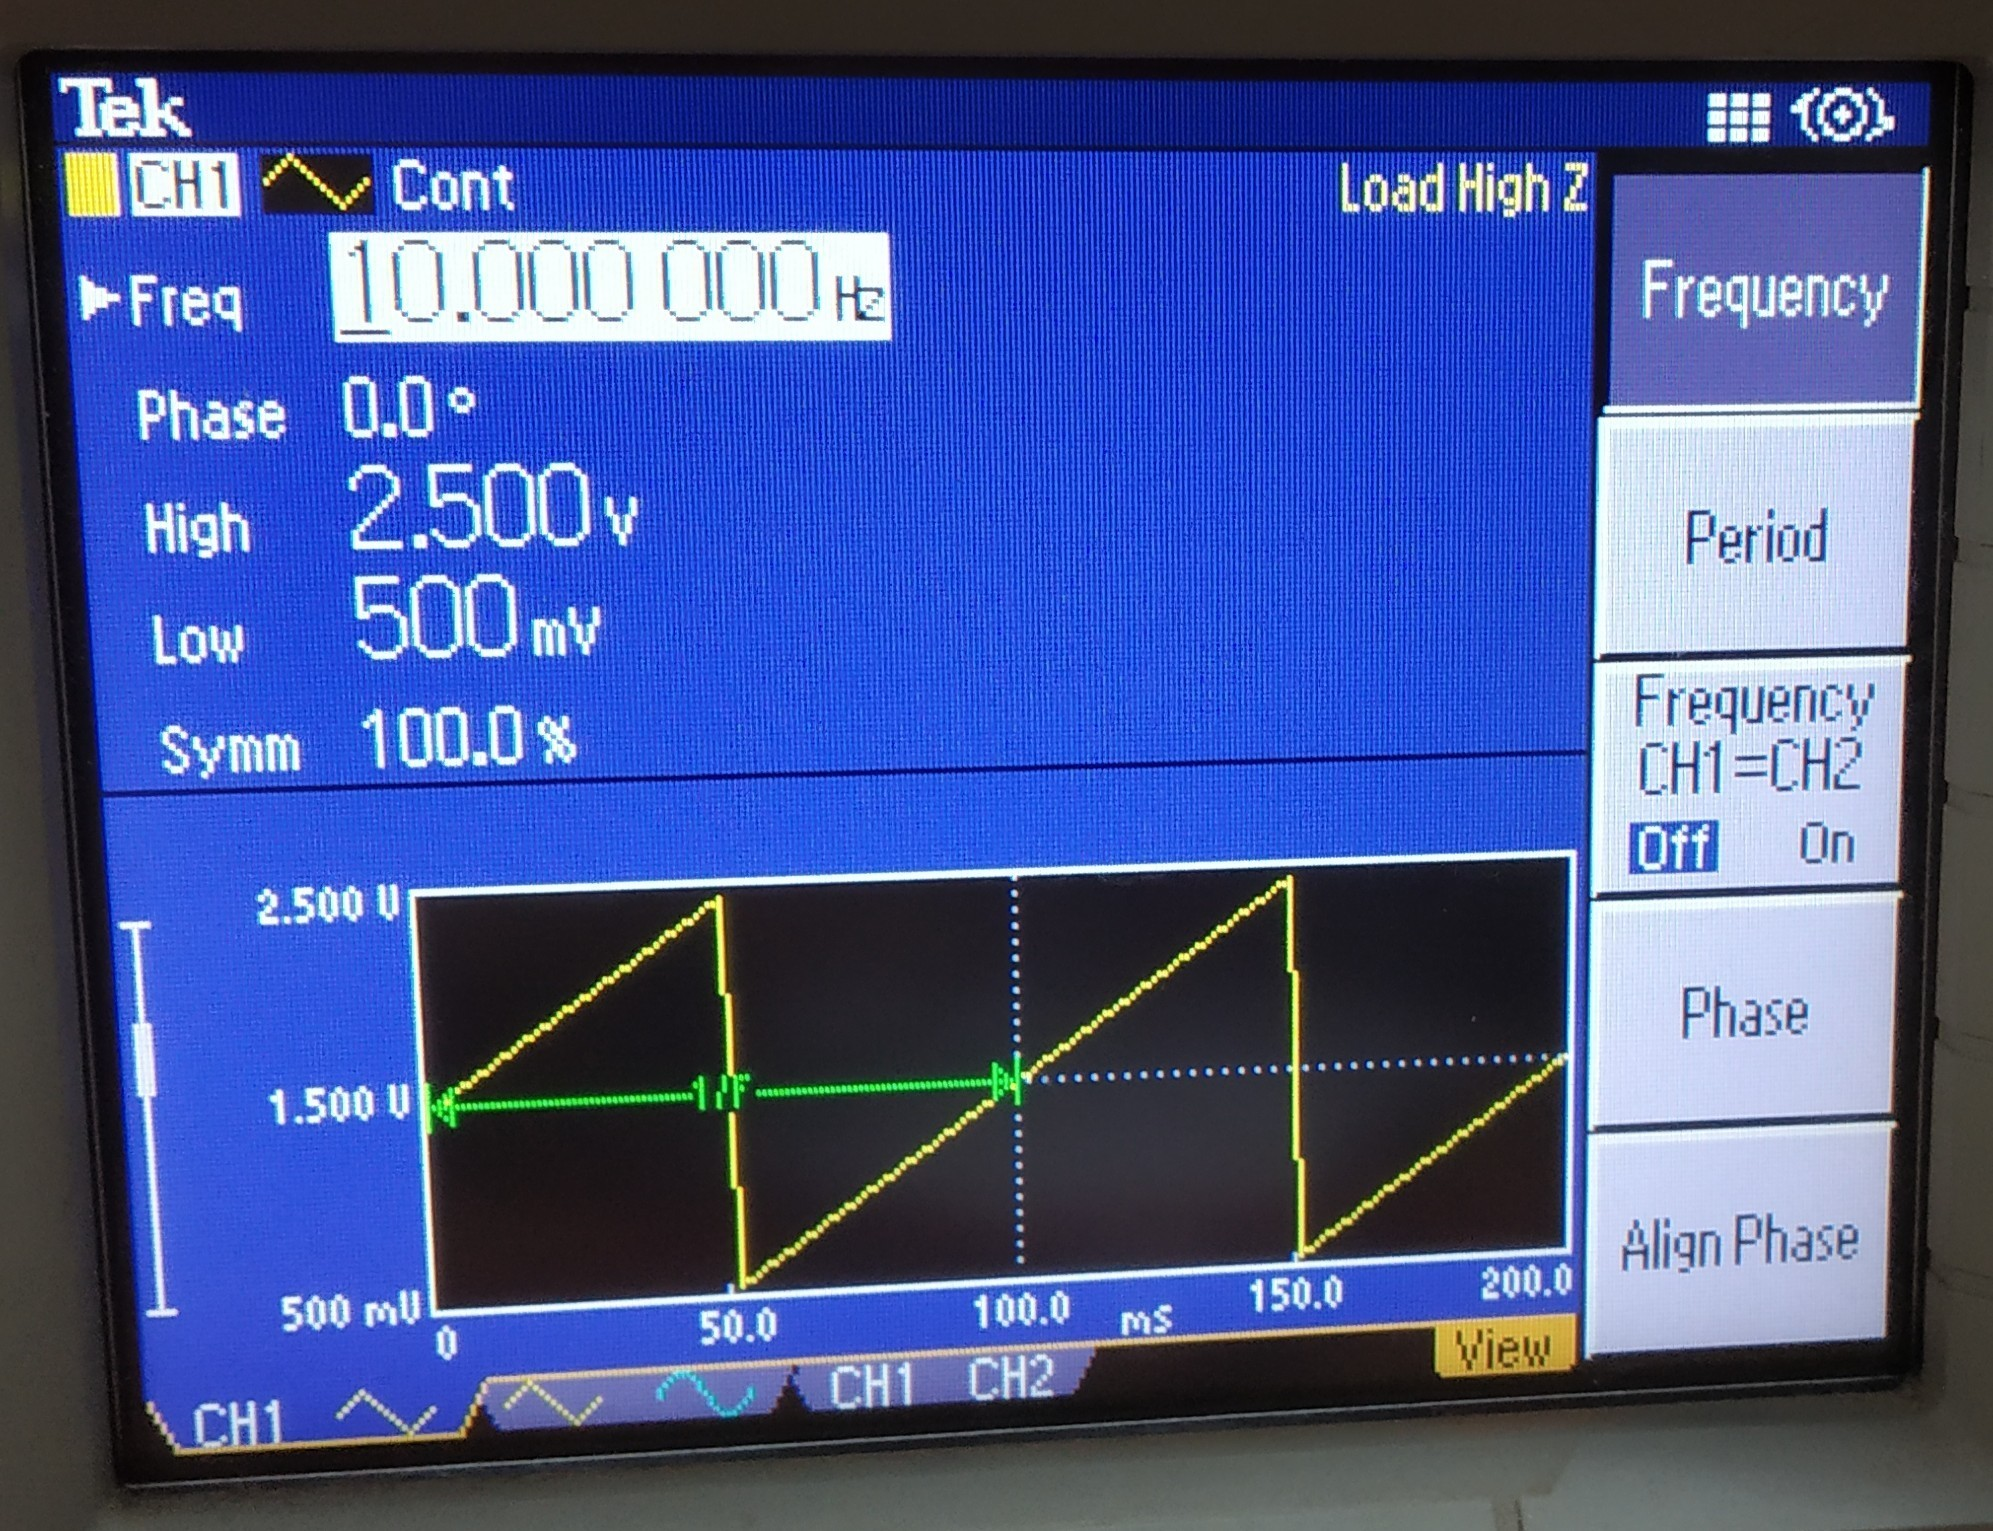
\includegraphics[width=70mm]{reports/lab5/ramp.jpg}
                \caption{Ramp signal}
            \end{subfigure}%
            \begin{subfigure}{.5\textwidth}
                \centering
                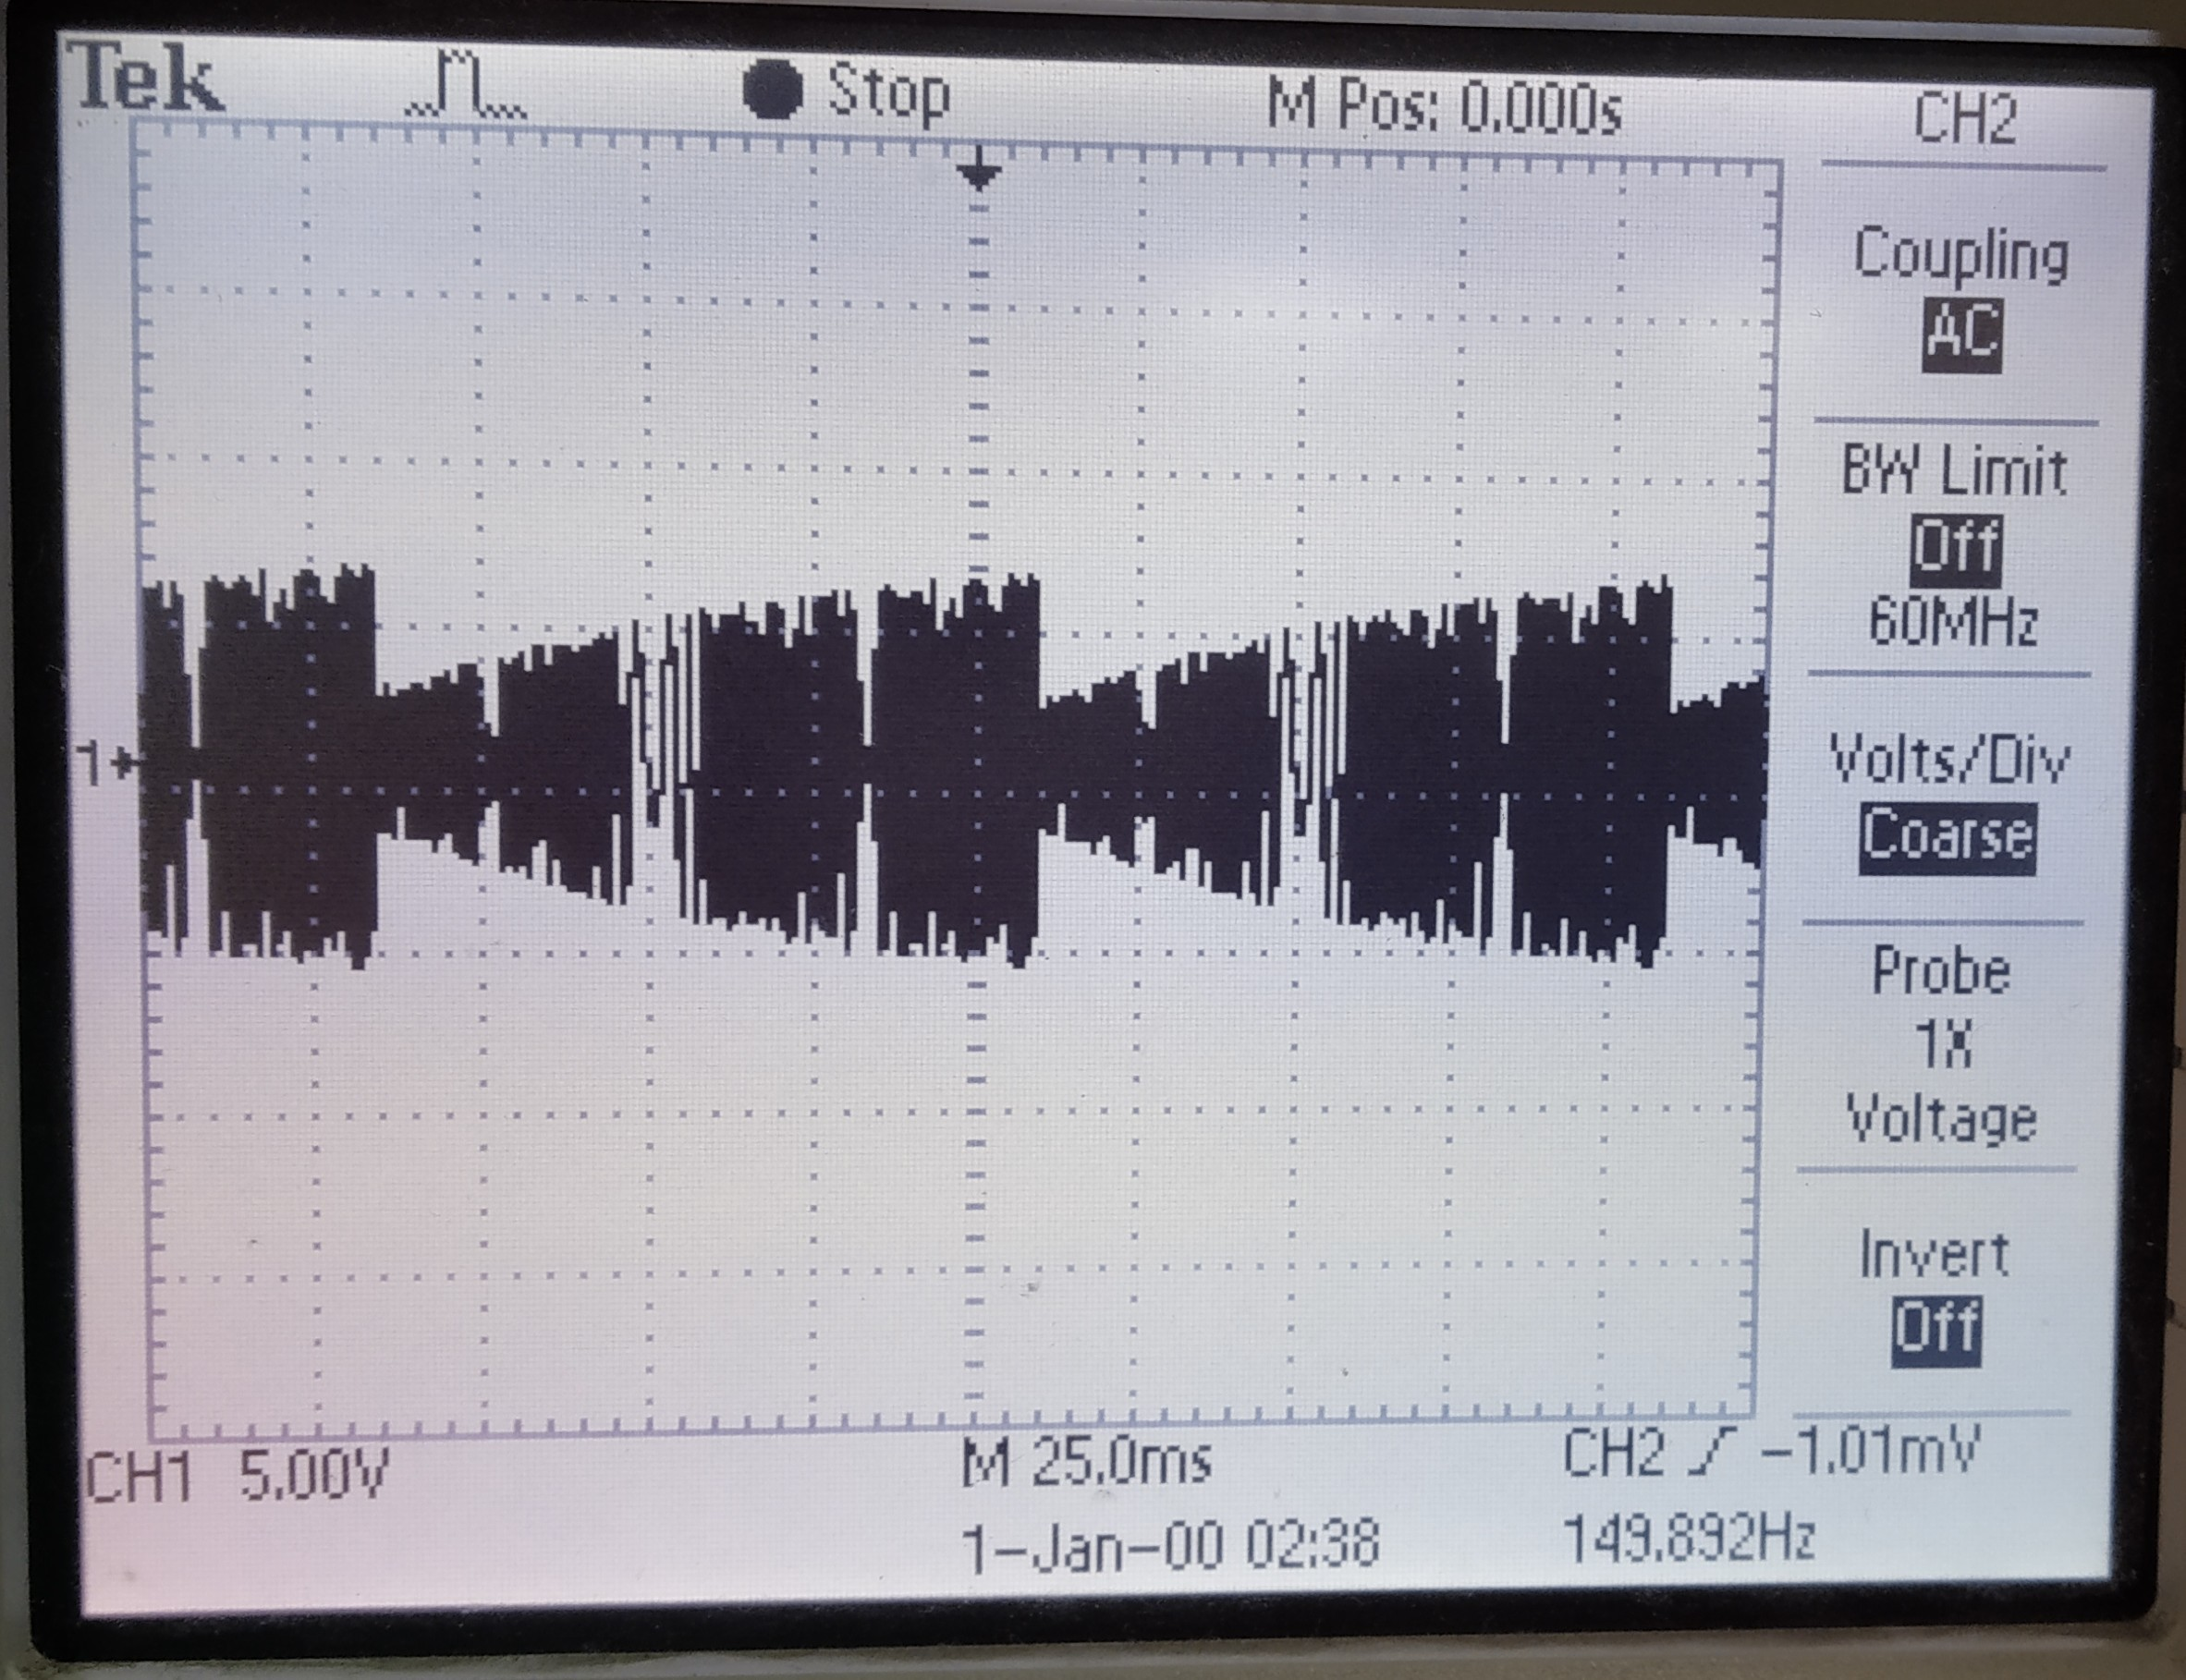
\includegraphics[width=70mm]{reports/lab5/highpassfilter.jpg}
                \caption{Frequency Response of ramp signal}
            \end{subfigure}%
        \end{figure}
    \newpage
%%%%%%%%%%%%%%%%%%%%%%%%%%%%%%%%%%%%%%%%%%%%%%%%%%%%%%%%%%%%%%%%%%%%%%%%%%%%%%%%%%
\section{In-Lab Circuit}
    \begin{figure}[H]
        \centering
        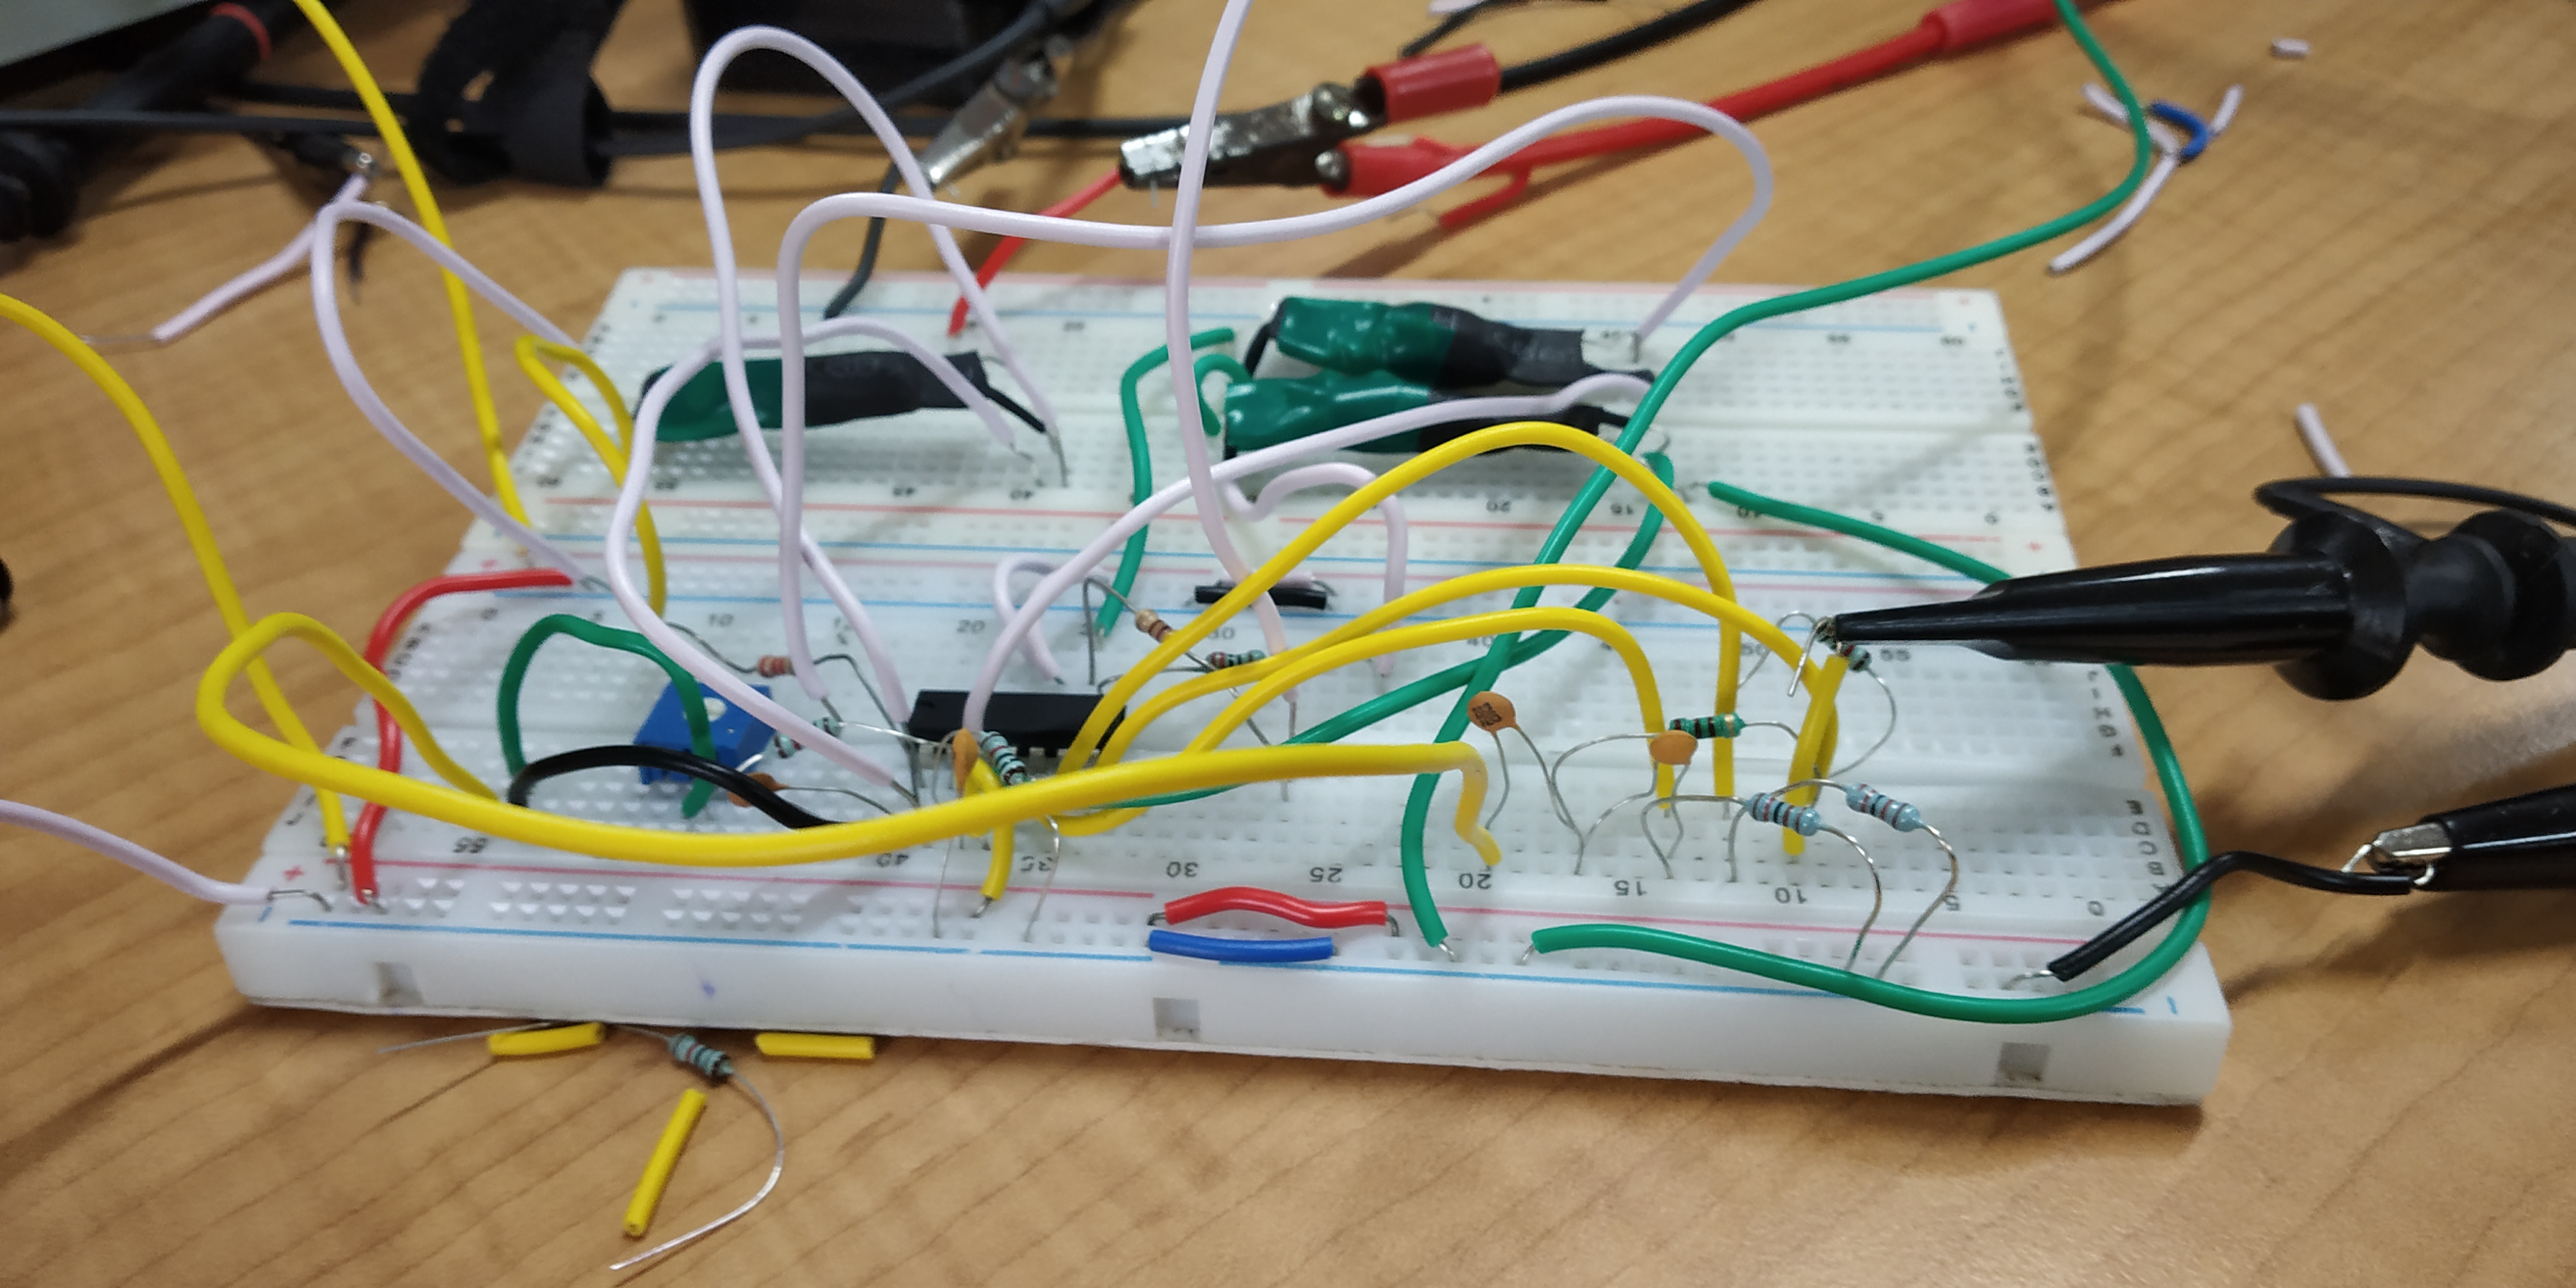
\includegraphics[width = 0.5\linewidth]{reports/lab5/inLab_ckt2.jpg}
        \caption{Bread-board circuit of Sweep generator with High Pass Filter}
    \end{figure}
    
%%%%%%%%%%%%%%%%%%%%%%%%%%%%%%%%%%%%%%%%%%%%%%%%%%%%%%%%%%%%%%%%%%%%%%%%%%%%%%%%%%%
\vspace{4cm}

    \begin{thebibliography}{9}

        \bibitem{Analog LAB Manual} 
        Experiment Handout
        \\\texttt{http://wel.ee.iitb.ac.in/teaching\_labs/WEL\%20Site/ee230/Labsheets-2020/\\Handouts/lab5\_handout\_observing\_frequency\_response\_of\_a\_filter\_in\_time\_\\domain\_modified\_14\_02\_2020.pdf}
        \bibitem{Supporting material}
        Supporting material for Wien Bridge Oscillator and High Pass Filter
        \\\texttt{http://wel.ee.iitb.ac.in/teaching\_labs/WEL\%20Site/ee230/Labsheets-2020/\\supporting\_documents/Freq\_resp\_on\_DSO.zip}
        \bibitem{Datasheet of TL084}
        Data-sheet of op-amp TL084
        \\\texttt{https://www.ti.com/lit/ds/symlink/tl082b.pdf\\?HQS=TI-null-null-alldatasheets-df-pf-SEP-wwe}
        
    \end{thebibliography}

\end{document}

%%%%%%%%%%%%%%%%%%%%%%%%%%%%%%%%%%%%%%%%%%%%%%%%%%%%%%%%%%%%%%%%%%%%%%%%%%%%%%%%%%%%%%%%%%%%%%%%%%%%%%%%%%%%%